\documentclass[12pt,a4paper]{report}

\usepackage[utf8]{inputenc}
\usepackage[T1]{fontenc}
\usepackage[spanish,es-noshorthands]{babel}
\usepackage{csquotes} 
\usepackage{graphicx}

\usepackage{tabularx}
\usepackage{makecell}
\usepackage{multirow}
\usepackage{array}
\usepackage{cellspace}
\usepackage{listings}
\usepackage{xcolor}
\usepackage{amsmath}

\usepackage{tcolorbox}
\usepackage{listings}

\usepackage{longtable}
\usepackage{booktabs}
\usepackage{array}


% Define JSON language
\definecolor{delim}{RGB}{20,105,176}
\definecolor{numb}{RGB}{106, 109, 32}
\definecolor{string}{rgb}{0.64,0.08,0.08}

% JSON-specific configuration
\lstdefinelanguage{JSON}{
  string=[s]{"}{"},
  stringstyle=\color{red},
  comment=[l]{:},
  commentstyle=\color{blue},
  keywords={false,true,null},
  keywordstyle=\color{purple}\bfseries,
  morecomment=[l]{//},
  morecomment=[s]{/*}{*/},
  morestring=[b]',
  morestring=[b]",
  sensitive=false
}

\lstset{
  language=JSON,
  backgroundcolor=\color{gray!5},
  basicstyle=\ttfamily\footnotesize,
  breaklines=true,
  breakatwhitespace=true,
  columns=fullflexible,
  showstringspaces=false,
  frame=single,
  frameround=tttt,
  framesep=5pt,
  numbers=left,
  numberstyle=\tiny\color{gray},
  numbersep=10pt,
  tabsize=2,
  literate=
    {,}{{\color{blue},}}1
    {:}{{\color{blue}:}}1
    {\{}{{\color{darkgray}\{}}1
    {\}}{{\color{darkgray}\}}}1
    {[}{{\color{darkgray}[}}1
    {]}{{\color{darkgray}]}}1,
}

\lstdefinelanguage{CSV}{
  string=[s]{"}{"},
  stringstyle=\color{red},
  comment=[l]{\#},
  commentstyle=\color{gray},
  keywords={},
  morecomment=[l]{//},
  morestring=[b]',
  morestring=[b]",
  sensitive=false
}

\lstset{
  language=CSV,
  backgroundcolor=\color{gray!5},
  basicstyle=\ttfamily\footnotesize,
  breaklines=true,
  breakatwhitespace=true,
  columns=fullflexible,
  showstringspaces=false,
  frame=single,
  frameround=tttt,
  framesep=2pt,
  numbers=left,
  numberstyle=\tiny\color{gray},
  numbersep=5pt,
  tabsize=2,
  literate=
    {,}{{\color{blue},}}1
    {\{}{{\color{darkgray}\{}}1
    {\}}{{\color{darkgray}\}}}1
    {[}{{\color{darkgray}[}}1
    {]}{{\color{darkgray}]}}1,
}

\lstdefinelanguage{SQL}{
  keywords={CREATE, SELECT, INSERT, UPDATE, DELETE, FROM, WHERE, AND, OR, 
    NOT, ORDER, BY, GROUP, HAVING, JOIN, INNER, OUTER, LEFT, RIGHT, FULL, 
    ON, AS, UNION, ALL, IN, IS, NULL, LIKE, BETWEEN, EXISTS, CASE, WHEN, 
    THEN, ELSE, END, WITH, TABLE, VIEW, FUNCTION, PROCEDURE, TRIGGER, 
    DATABASE, SCHEMA, INDEX, PRIMARY, KEY, FOREIGN, REFERENCES, 
    CONSTRAINT, UNIQUE, CHECK, DEFAULT, ALTER, DROP, TRUNCATE, GRANT, 
    REVOKE, COMMIT, ROLLBACK, BEGIN, TRANSACTION, SET, VALUES, TOP, 
    LIMIT, OFFSET, ASC, DESC, DISTINCT, COUNT, SUM, AVG, MIN, MAX, INTO},
  sensitive=true,
  morecomment=[l]--,
  morecomment=[s]{/*}{*/},
  morestring=[b]',
  morestring=[b]",
}

\lstset{
 language=SQL,
 backgroundcolor=\color{gray!5},
 basicstyle=\fontfamily{lmtt}\selectfont\footnotesize,
 keywordstyle=\color{blue!80!black},
 identifierstyle=\color{black},
 commentstyle=\color{green!60!black},
 stringstyle=\color{red!70!black},
 numberstyle=\tiny\color{gray!70},
 numbers=left,
 stepnumber=1,
 breaklines=true,
 breakatwhitespace=false,
 showstringspaces=false,
 tabsize=2,
 captionpos=b,
 frame=single,
 frameround=tttt,
 rulecolor=\color{gray!50},
 framesep=3pt,
 xleftmargin=5pt,
}


\usepackage{tikz}
\usetikzlibrary{shapes,arrows,positioning}

% Load biblatex with Spanish options
\usepackage[spanish]{babel}
\usepackage{csquotes}
\usepackage[
  backend=biber,
  style=ieee,          % Estilo IEEE, muy usado en informática
  giveninits=true,     % Usa iniciales para nombres
  maxcitenames=3,      % Usa "et al." después de 3 autores en citas
  maxbibnames=3,       % Muestra hasta 6 autores en la bibliografía
  mincitenames=1,      % Mínimo 1 autor antes de "et al."
  uniquelist=false,    % No intenta hacer listas de autores únicas
  uniquename=false,    % No intenta hacer nombres únicos
  minbibnames=3,       % Mínimo 3 autores en bibliografía antes de "et al."
  sorting=nyt,         % Ordena por nombre, año, título
  url=false,           % No muestra URLs en entradas que tienen DOI
  doi=true,            % Muestra DOIs
  isbn=false,          % No muestra ISBN en la bibliografía
  dashed=false,        % No usa guiones para autores repetidos
  urldate=comp,        % Formato compacto para fechas de acceso
  useprefix=false      % Maneja correctamente prefijos en apellidos como "de
]{biblatex}

% Traducir "et al." a "y otros" en español
\DefineBibliographyStrings{spanish}{
  andothers = {y otros},
}
\renewcommand*{\bibinitperiod}{.}
\renewcommand*{\bibinitdelim}{\addnbthinspace}

\DeclareNameFormat{given-family}{%
  \ifgiveninits
    {\usebibmacro{name:given-family}
      {\namepartfamily}
      {\namepartgiveni}
      {\namepartprefix}
      {\namepartsuffix}}
    {\usebibmacro{name:given-family}
      {\namepartfamily}
      {\namepartgiven}
      {\namepartprefix}
      {\namepartsuffix}}%
  \usebibmacro{name:andothers}}

% Add your bibliography file
\addbibresource{references.bib}

\begin{document}

% Carátula
\begin{titlepage}
    \centering
    {\huge\bfseries Comparación de las arquitecturas Kappa y Delta para el monitoreo remoto de pacientes basado en datos de sensores \par}
    \vspace{2cm}
    {\Large Entregado como requisito para la obtencion del
titulo de Master en Big Data\par}
    \vspace{1cm}
    {\large Emiliano Conti - \par}
    \vspace{1cm}
    {\large Tutor: Alejandro Bianchi \par}
    \vspace{1cm}
    {\small Universidad ORT\par}
    \vspace{1cm}
    {\large \today\par}
\end{titlepage}

% Disclaimer

\thispagestyle{empty}

\begin{center}
    \Large\bfseries Disclaimer
\end{center}
\vspace{1cm}

\noindent Yo, Emiliano Conti declaro que el trabajo que se presenta en esta obra es de mi propia mano. Puedo asegurar que:

\begin{itemize}
    \item La obra fue producida en su totalidad mientras realizaba el Proyecto Final del Master en Big Data;
    \item Cuando he consultado el trabajo publicado por otros, lo he atribuido con claridad;
    \item Cuando he citado obras de otros, he indicado las fuentes. Con excepci\'on de estas citas, la obra es enteramente m\'ia;
    \item En la obra, he acusado recibo de las ayudas recibidas;
    \item Cuando la obra se basa en trabajo realizado conjuntamente con otros, he explicado claramente qu\'e fue contribuido por otros, y qu\'e fue contribuido por mi;
    \item Ninguna parte de este trabajo ha sido publicada previamente a su entrega, excepto donde se han realizado las aclaraciones correspondientes.
\end{itemize}

\vspace{2cm}

\noindent Firma: \rule{5cm}{0.1pt}

\vspace{1cm}

\noindent Fecha: \rule{5cm}{0.1pt}

% Abstract
\renewcommand{\abstractname}{Abstract}
\begin{abstract}
    En el contexto del monitoreo remoto de pacientes, 
    el procesamiento eficiente y confiable de datos de sensores en tiempo real se vuelve un requisito fundamental para la prevención y mejora de la atención médica. 
    
    Este trabajo analiza y compara dos arquitecturas modernas de procesamiento de datos en streaming: \textit{Kappa} y \textit{Delta}, 
    con el objetivo de determinar cuál resulta más adecuada para este tipo de sistemas.

    Se desarrolló un sistema de monitoreo basado en sensores que simula un entorno hospitalario y utiliza puntuaciones derivadas del sistema \textit{NEWS2} para evaluar el estado de salud de los pacientes. 
    Sobre este entorno se implementaron ambas arquitecturas utilizando un stack tecnológico compuesto por herramientas como Apache Kafka, Apache Flink y Apache Doris, entre otras.

    La comparación se realizó en función de métricas técnicas como latencia, throughput, uso de recursos y tolerancia a fallos, 
    así como también aspectos operativos y de costo. 
    
    Los resultados muestran que la arquitectura \textit{Kappa} ofrece menores tiempos de latencia, 
    mientras que la arquitectura \textit{Delta} destaca por su alto throughtput, escalabilidad, gestión operativa 
    y flexibilidad para reprocesamiento histórico y mejor integración con almacenamiento analítico.

    Finalmente, se discuten los desafíos asociados a la implementación de estas arquitecturas en entornos de salud, 
    y se presentan recomendaciones para su adopción según las necesidades específicas del sistema.
\end{abstract}

% Índice
\tableofcontents

\setcounter{page}{5}
% Capítulos
\chapter{Introducción}


\section{Descripción del Proyecto}

Este proyecto compara las arquitecturas Kappa y Delta en el contexto del monitoreo remoto de pacientes mediante sensores IoT. En la era de la salud digital, estos sistemas generan grandes volúmenes de datos en tiempo real que requieren procesamiento eficiente. Se analizarán ambas arquitecturas, se definirán métricas de comparación y se implementarán en un caso de uso de monitoreo de pacientes. El objetivo es determinar la arquitectura más adecuada, considerando factores como latencia, escalabilidad, complejidad de implementación y manejo de datos históricos y en tiempo real.

\newpage

\section{Objetivos}

\begin{enumerate}
    \item Realizar un análisis teórico exhaustivo de las arquitecturas Kappa y Delta, detallando sus componentes y flujos de datos.
    
    \item Definir un conjunto de métricas y criterios para la comparación objetiva de ambas arquitecturas en el contexto del monitoreo remoto de pacientes.
    
    \item Implementar ambas arquitecturas utilizando un conjunto de datos simulado de sensores de monitoreo de pacientes.
    
    \item Ejecutar pruebas de rendimiento y funcionalidad en ambas implementaciones.
    
    \item Analizar los resultados obtenidos y determinar la arquitectura más adecuada para el caso de uso específico de monitoreo remoto de pacientes.
\end{enumerate}

\newpage

\section{Caso de Estudio: Big Data en Sistema de Salud}

\subsection{Contexto del Sistema}
Sistema de salud integral que incluye perfiles de pacientes, telemedicina e integración con dispositivos IoT. El objetivo es mejorar la atención médica, con foco en prevenciín, utilizando tecnología.

\subsection{Descripción del Caso de Uso}
Monitoreo continuo y en tiempo real de la salud del paciente mediante el uso de Big Data. Se espera ademas, tener la capacidad de identificar patrones y tendencias en los datos médicos. Así como también proporcionar recomendaciones personalizadas.

\subsection{Proceso}
\begin{enumerate}
    \item \textbf{Recopilación de Datos}:
    \begin{itemize}
        \item Dispositivos IoT (datos en tiempo real)
    \end{itemize}
    
    \item \textbf{Almacenamiento y Gestión}:
    \begin{itemize}
        \item Almacenamiento de datos centralizada, segura y escalable
    \end{itemize}
    
    \item \textbf{Análisis de Datos}:
    \begin{itemize}
        \item Procesamiento en tiempo real
        \item Análisis históricos
    \end{itemize}
    
    \item \textbf{Generación de Insights}:
    \begin{itemize}
        \item Tableros
        \item Alertas en tiempo real
    \end{itemize}
    
    \item \textbf{Intervención y Seguimiento}:
    \begin{itemize}
        \item Monitoreo continuo
        \item Feedback y mejora continua del sistema
    \end{itemize}
\end{enumerate}
\chapter{Marco Teórico}

\section{Introducción a Big Data y Streaming de Datos}

\subsection{Sistemas Distribuidos}
Un sistema distribuido es una colección de elementos computacionales autonomos que para su usuario 
parecen un sistema único y coherente. \parencite{tanenbaum}

Los sistemas distribuidos tienen dos caracteristicas que pueden regularse para escalar: Procesamiento y Almacenamiento. 
\newline

En el último tiempo, ha habido una tendencia a preferir que la escala de ambas propiedades sea individual. 
Es decir, que se pueda escalar por un lado la potencia de procesamiento y por otro la capacidad de almacenamiento.

\subsubsection{Consistencia}
La Consistencia es la propiedad que tiene un sistema distribuido en la que todos los nodos ven los mismos datos al mismo tiempo.
Esto significa que cualquier lectura en cualquier momento deberá devolver el valor más reciente escrito para ese dato.
Si un sistema es consistente, una vez que se realiza una escritura, todas las lecturas subsiguientes deben reflejar esa escritura;
sin importar desde que nodo se hagan. 
Esta propiedad garantiza que los clientes de los sistemas nunca vean datos desactualizados o inconsistentes.
\newpage
\subsubsection{Disponibilidad}
La Disponibilidad es la propiedad que tiene un sistema distribuido para responder a todas las peticiones, ya sean de lectura o escritura, sin fallos.
Un sistema disponible garantiza que cada solicitud reciba una respuesta sin importar el estado individual de cada nodo que lo compone.
Esto significa que incluso si algunos nodos falla, el sistema en su conjunto debe poder seguir dando servicio a las peticiones que recibe.
\subsubsection{Tolerancia a Particiones}
La Tolerancia a Particiones es la propiedad que tiene un sistema distribuido en la que continua funcionando a pesar de la perdida de 
conectividad entre nodos. Una partición ocurre cuando hay una ruptura en la comunicación dentro de la red, 
lo que resulta en que dos o más segmentos de la red no puedan comunicarse entre sí.
Un sistema tolerante a particiones puede seguir operando incluso cuando estas particiones ocurren, 
lo que significa que puede manejar retrasos o pérdidas de mensajes entre nodos sin fallar por completo. 

\newpage
\subsection{Definición y características del Big Data}

Big Data es un término paraguas que se usa para denominar a un conjunto de tecnologías que manejan grandes volúmenes de datos.
La pregunta que se presenta entonces es: ¿qué tan grandes deberían ser estos volúmenes para ser considerados Big Data?
O incluso, ¿existen otras características que definan lo que es Big Data?
Una definición generalmente aceptada es la siguiente:
\bigskip

Las tecnologías de Big Data están orientadas a
procesar datos de alto volumen, alta velocidad y alta variedad
para extraer el valor de datos previsto y asegurar una alta
veracidad de los datos originales y la información obtenida, lo que demanda
formas de procesamiento de datos e información rentables e innovadoras
para mejorar el conocimiento, la toma de decisiones y el control de procesos. \newline

Todo esto exige nuevos modelos de datos
que soporten todos los estados y etapas de los datos durante todo su ciclo de vida, 
y nuevos servicios y herramientas de infraestructura que permitan obtener y procesar
datos de una variedad de fuentes y
entregar datos en una variedad de formas a diferentes consumidores y dispositivos
de datos e información. \parencite{demchenko2014addressing}

\newpage
Por lo que podríamos considerar que es Big Data todo aquello que esté orientado a datos
cuyo volumen, velocidad y variedad no puedan ser tratados por un modelo de procesamiento
de datos tradicional (como podrían ser las bases de datos relacionales). Con el objetivo
de generar valor, asegurando la veracidad de los datos originales y la información obtenida.

\subsection{Streaming de datos}

El streaming de datos, también conocido como procesamiento de flujo, es un paradigma 
de procesamiento de datos en el que los datos se tratan como un flujo continuo e 
ilimitado de eventos discretos. En el contexto de Big Data, el streaming permite procesar 
y analizar grandes volúmenes de datos en tiempo real o casi real, a medida que se generan 
o llegan al sistema. \parencite{flink}

\subsection{Teorema CAP}
El Teorema CAP es un concepto fundamental en el diseño de sistemas distribuidos. 
Este establece que es imposible garantizar al mismo tiempo, tanto la Consistencia (Consistency), 
Disponibilidad (Availability) y la Tolerancia a las Particiones (Partition Tolerance).\newline

Según esto, un sistema distribuido sólo es capaz de garantizar dos de estas propiedades al mismo tiempo. 
En general, para los sistemas de Big Data de Streaming, la disponibilidad es una propiedad obligatoria, ya que cualquier inactividad puede 
resultar en la pérdida de datos valiosos o en la imposibilidad de realizar acciones.\newline

Por otro lado, la Tolerancia a Particiones es también indispensable para estos sistemas, que por su naturaleza requieren que su capacidad de 
procesamiento este distribuida a través de múltiples nodos dispersos en una red no confiable; por lo que son suceptibles 
a que se genere una partición. Por lo tanto, si no tuviera esta propiedad el servicio podría dejar de ser disponible.\newline 

Entonces, como corolario, un sistema de Big Data de Streaming debe también ser tolerante a las particiones para poder ser disponible.
Esto nos deja con una única opción: relajar el "grado de consistencia" hasta un punto razonable que permita que el sistema siga siendo eficáz.\parencite{capteo}
\newpage
\subsubsection{Consistencia Eventual}
La consistencia eventual es un modelo de consistencia en sistemas distribuidos que garantiza que, 
si no se realizan nuevas actualizaciones a un objeto, en algun momento (eventualmente) todos los accesos a ese objeto 
devolverán el último valor actualizado. \newline

La consistencia eventual se alinea con las compensaciones descritas por el teorema CAP, 
permitiendo que estos sistemas prioricen la disponibilidad y la tolerancia a particiones. \newline

Además, facilita la escalabilidad horizontal, crucial para manejar el crecimiento continuo de datos y clientes de los sistemas.
Por último, es importante diseñar cuidadosamente el sistema para manejar las posibles inconsistencias temporales 
y asegurar que la aplicación pueda tolerar y resolver estas situaciones de manera apropiada \parencite{capteo}

\newpage

\subsection{Desafíos en el manejo de datos de streaming}

\begin{enumerate}
    \item \textbf{Procesamiento en tiempo real y baja latencia}
    
    El procesamiento de datos debe ocurrir con un retraso mínimo para proporcionar resultados en tiempo real.
    
    Un desafío clave en el streaming es lograr equilibrar la latencia, el costo y la correctitud simultáneamente \parencite{akidau2015dataflow}.

    \item \textbf{Manejo de datos fuera de orden}
    
    Los datos pueden llegar en un orden diferente al que fueron generados, lo que complica el procesamiento.
    
    El procesamiento de eventos fuera de orden es un desafío fundamental en los sistemas de streaming \parencite[p.~87]{flink}.

    \item \textbf{Escalabilidad}
    
    Los sistemas deben poder manejar volúmenes crecientes de datos sin degradación del rendimiento.
    
    La escalabilidad en sistemas de streaming implica la capacidad de aumentar el rendimiento añadiendo recursos computacionales \parencite{samurai}.

    \newpage
    \item \textbf{Tolerancia a fallos y consistencia}
    
    El sistema debe poder recuperarse de fallos sin pérdida de datos y mantener la consistencia eventual de los resultados.
    
    Garantizar la semántica de "exactly-once" en presencia de fallos es un desafío significativo en streaming \parencite{carbone2015apache}.

    \item \textbf{Procesamiento de ventanas temporales}
    
    Definir y procesar eficientemente ventanas de tiempo sobre streams de datos continuos.
    
    El procesamiento de ventanas temporales es fundamental en aplicaciones de streaming y requiere consideraciones cuidadosas en cuanto a la semántica del tiempo y la completitud de los datos \parencite{akidau2015dataflow}.

    \item \textbf{Integración con sistemas batch}
    
    Combinar eficazmente el streaming con sistemas batch existentes.
    
    La integración de paradigmas batch y streaming, a menudo referida como 'procesamiento híbrido', presenta desafíos únicos en términos de consistencia de datos y modelos de programación \parencite{carbone2015apache}.
\end{enumerate}
\newpage

\subsection{Conceptos clave en el procesamiento de streaming}

El procesamiento de streaming se refiere al análisis y manipulación de datos en tiempo real a medida que se generan o reciben. Según Carbone et al. \parencite{carbone2015apache}, los conceptos fundamentales incluyen:

\begin{itemize}
    \item \textbf{Flujo de datos}: Una secuencia potencialmente infinita de registros que llegan continuamente \parencite{akidau2015dataflow}.
    \item \textbf{Latencia}: El tiempo entre la llegada de un dato y su procesamiento, crucial para aplicaciones en tiempo real \parencite{akidau2015dataflow}.
    \item \textbf{Ventanas}: Mecanismos para agrupar datos en intervalos finitos para su procesamiento \parencite{akidau2015dataflow}.
    \item \textbf{Estado}: Información que se mantiene entre eventos para cálculos incrementales \parencite{carbone2015apache}.
    \item \textbf{Watermarks}: Indicadores de progreso del tiempo en el flujo de datos \parencite{akidau2015dataflow}.
\end{itemize}

\subsection{Comparación entre procesamiento por lotes y en tiempo real}

La elección entre procesamiento por lotes y en tiempo real depende de los requisitos específicos de la aplicación:

\begin{table}[h]
\centering
\begin{tabular}{|p{3cm}|p{5cm}|p{5cm}|}
\hline
\textbf{Característica} & \textbf{Procesamiento por lotes} & \textbf{Procesamiento en tiempo real} \\
\hline
Latencia & Alta (minutos a horas) & Baja (milisegundos a segundos) \\
\hline
Throughput & Alto & Moderado a alto \\
\hline
Complejidad & Menor & Mayor \\
\hline
Consistencia & Fuerte & Eventual \\
\hline
Uso típico & Análisis histórico, reportes & Monitoreo, alertas, decisiones inmediatas \\
\hline
\end{tabular}
\caption{Comparación de procesamiento por lotes y en tiempo real}
\label{tab:batch_vs_streaming}
\end{table}

Como sugiere Stonebraker et al. \parencite{stonebraker2005one}, el procesamiento en tiempo real es esencial para aplicaciones
que requieren decisiones inmediatas, mientras que el procesamiento por lotes es más 
adecuado para análisis profundos de grandes volúmenes de datos históricos.

\subsection{Evolución de las arquitecturas de procesamiento de datos}

La evolución de las arquitecturas de procesamiento de datos ha sido impulsada por la necesidad de manejar volúmenes cada vez mayores de datos en tiempo real:

\begin{enumerate}
    \item \textbf{Arquitecturas por lotes}: Sistemas tradicionales como Hadoop MapReduce, diseñados para procesar grandes volúmenes de datos estáticos \parencite{dean2008mapreduce}.
    \item \textbf{Arquitecturas de streaming puro}: Como Apache Storm, enfocadas en el procesamiento en tiempo real pero con limitaciones en la consistencia y exactitud \parencite{toshniwal2014storm}.
    \item \textbf{Arquitectura Lambda}: Propuesta por Marz \parencite{marz2011cap}, combina procesamiento por lotes y en tiempo real para balancear latencia, throughput y tolerancia a fallos.
    \item \textbf{Arquitectura Kappa}: Introducida por Kreps \parencite{kreps2014questioning}, simplifica la Lambda tratando todos los datos como streams.
    \item \textbf{Arquitectura Delta}: Desarrollada por Databricks, combina las ventajas de las arquitecturas Lambda y Kappa, optimizando el procesamiento de datos tanto en batch como en streaming \parencite{deltalake} \parencite{delta}.
\end{enumerate}
\newpage
\section{Arquitectura Lambda}

\subsection{Descripción General}
La Arquitectura Lambda es un paradigma de procesamiento de datos diseñado para manejar grandes cantidades de información en sistemas de Big Data. 
Propuesta por Nathan Marz en 2011, esta arquitectura busca abordar las limitaciones de los sistemas de procesamiento por lotes (batch) y en tiempo real, 
combinando ambos enfoques para proporcionar una vista completa y actualizada de los datos.

\subsection{Componentes Principales}
La Arquitectura Lambda se compone de tres capas fundamentales:

\subsubsection{Batch Layer}
\begin{itemize}
\item Almacena el conjunto completo de datos históricos.
\item Procesa periódicamente volúmenes arbitrarios de datos.
\item Genera vistas pre-computadas para consultas eficientes.
\end{itemize}

\subsubsection{Serving Layer}
\begin{itemize}
\item Almacena las vistas pre-computadas de la capa de lotes.
\item Proporciona acceso de baja latencia a los resultados.
\end{itemize}

\subsubsection{Speed Layer}
\begin{itemize}
\item Procesa datos en tiempo real.
\item Genera vistas de estos datos.
\item Mantiene los datos guardados unicamente hasta que la Batch Layer haya hecho el reprocesamiento de los datos historicos.
\end{itemize}

\newpage
\subsubsection{Vista Lógica}
\begin{figure}[h]
\centering
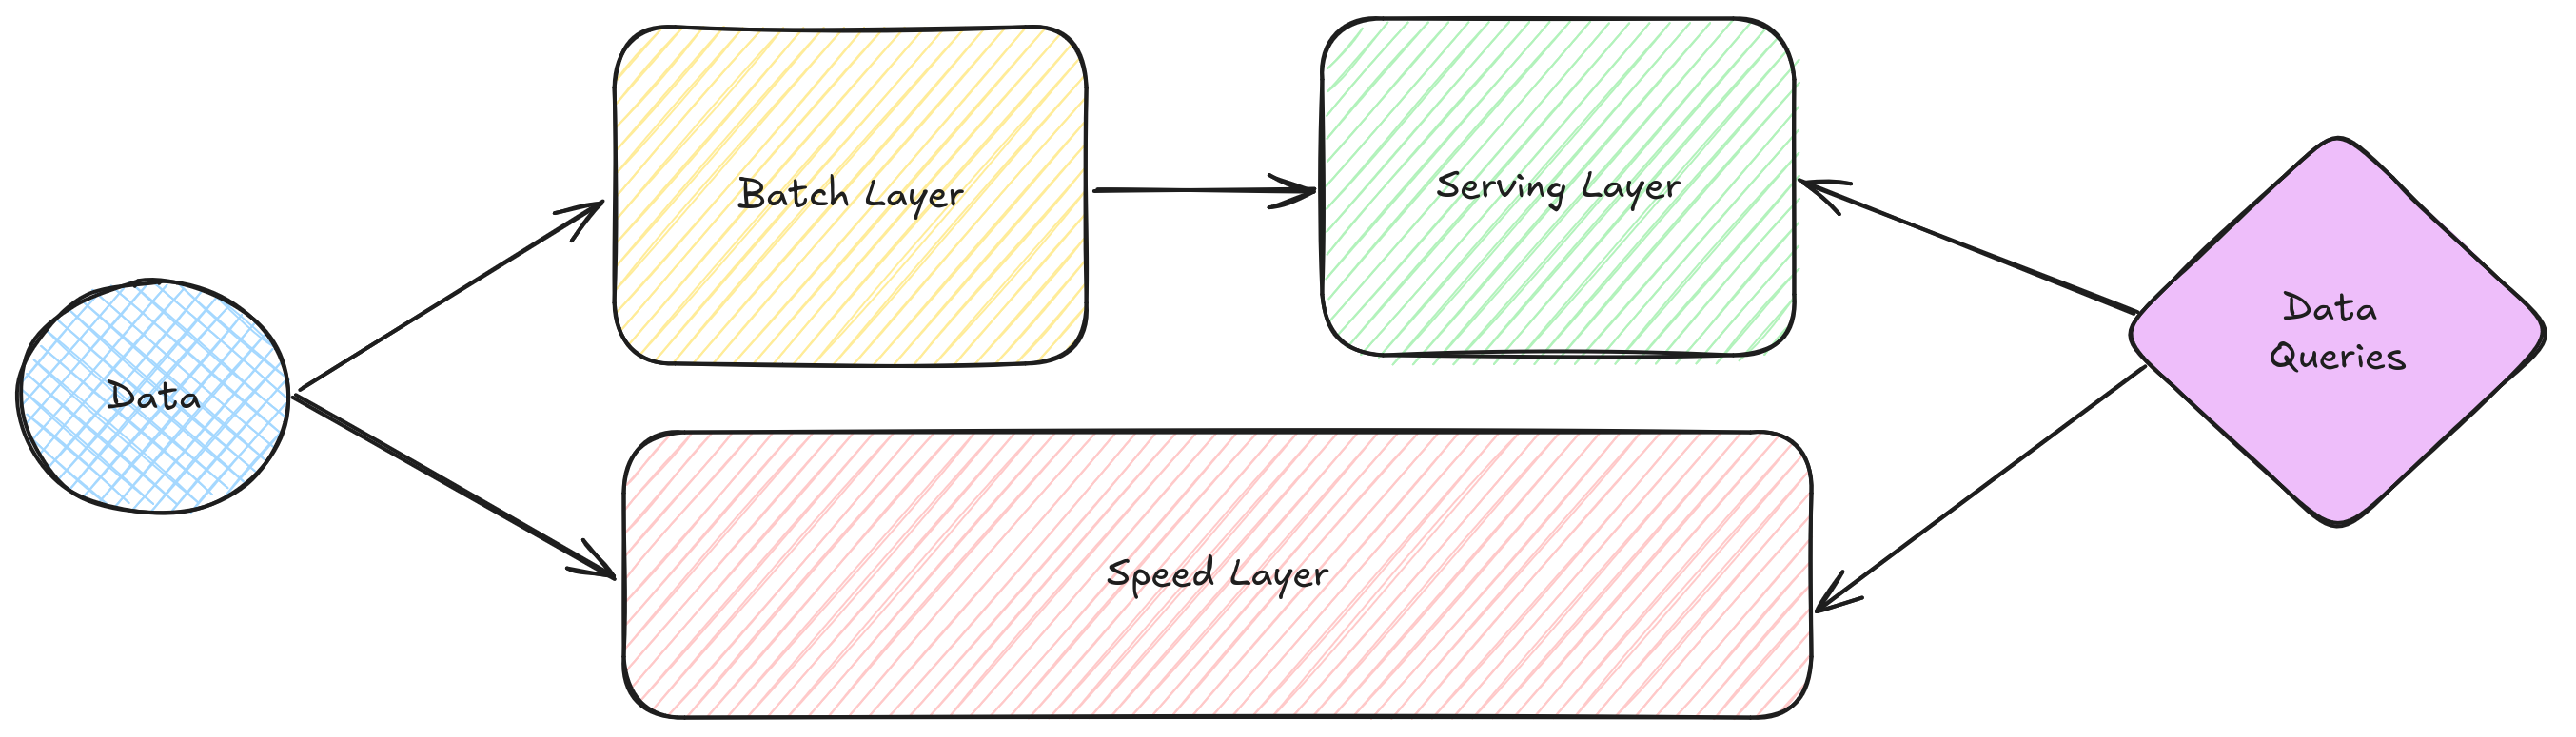
\includegraphics[width=0.8\textwidth]{teorico/lambda.png}
\caption{Diagrama de la Arquitectura Lambda}
\label{fig:arquitectura_lambda}
\end{figure}

\subsubsection{Implementación Típica}
\begin{figure}[h]
\centering
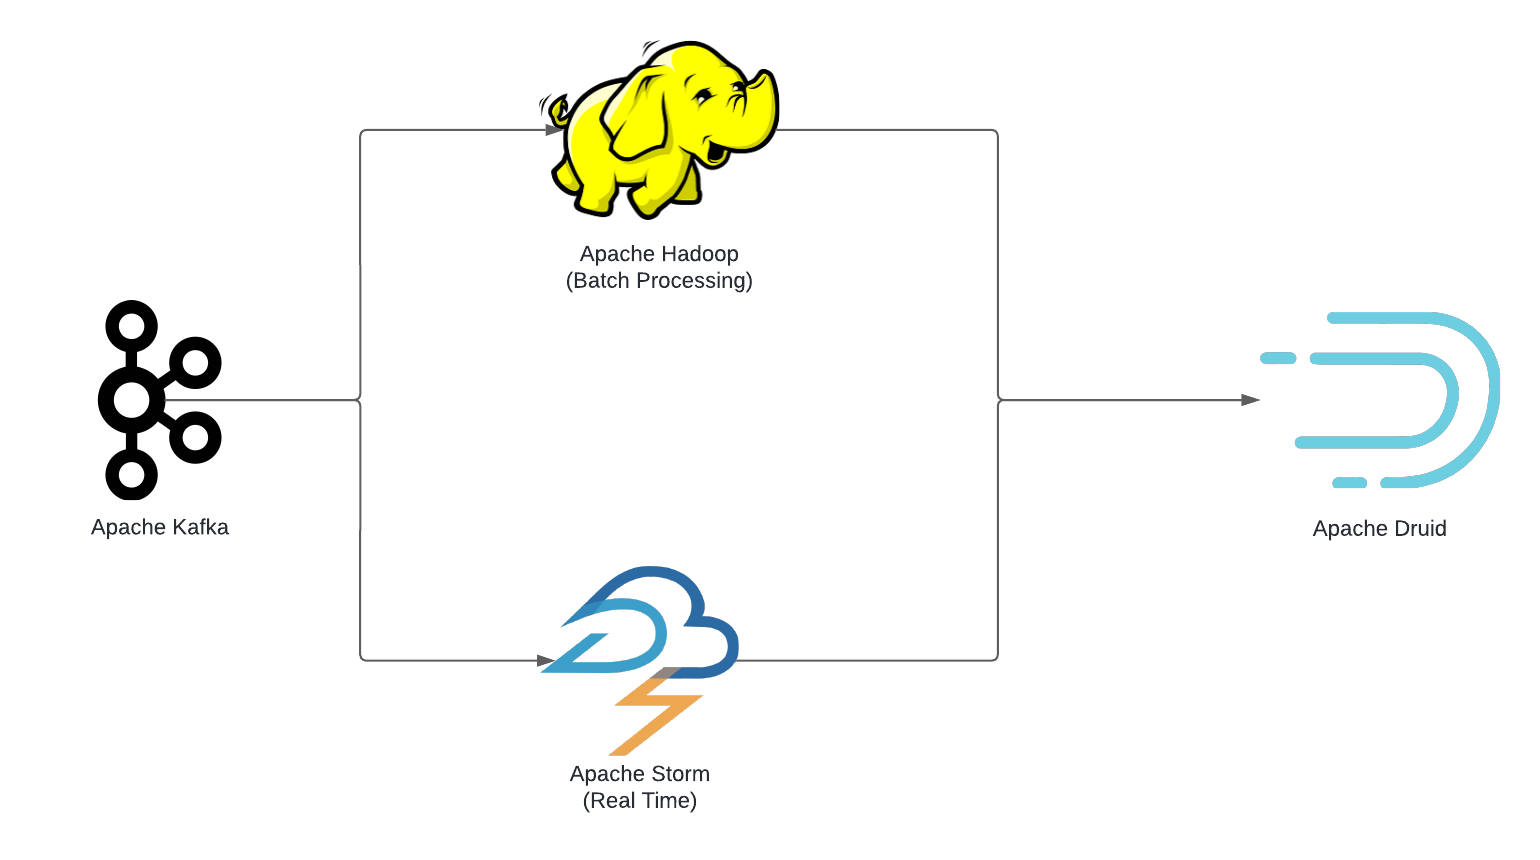
\includegraphics[width=0.8\textwidth]{teorico/LambdaImplement.png}
\caption{IMplementacion de la Arquitectura Lambda}
\label{fig:implementation_arquitectura_lambda}
\end{figure}



\subsection{Capacidades}
\begin{itemize}
\item \textbf{Procesamiento de datos a gran escala}: Maneja eficientemente volúmenes masivos de datos.
\item \textbf{Baja latencia}: Proporciona resultados en tiempo real para consultas.
\item \textbf{Tolerancia a fallos}: Mantiene la integridad de los datos incluso en caso de fallos del sistema.
\item \textbf{Escalabilidad}: Se adapta fácilmente al crecimiento del volumen de datos.
\item \textbf{Flexibilidad}: Permite el procesamiento tanto por lotes como en tiempo real.
\item \textbf{Consistencia eventual}: Garantiza que los datos eventualmente reflejarán todos los cambios.
\item \textbf{Reprocesamiento}: En caso de necesitar reprocesar los datos, este proceso es trivial, pues se tiene almacenado el histórico completo.
\end{itemize}

\subsection{Desafíos}
\begin{itemize}
\item \textbf{Complejidad}: La implementación y mantenimiento pueden ser complejos debido a la duplicación de lógica en las capas de lotes y velocidad.
\item \textbf{Latencia}: El procesamiento batch genera latencia debido al tiempo de la actualización de vistas.
\item \textbf{Costo}: Al utilizar recursos computacionales diferentes entre el procesamiento batch y en stream, esto puede requerir varios nodos computacionales, lo que incrementa los costos.
\end{itemize}

\subsection{Conclusiones}
La Arquitectura Lambda ofrece una solución robusta para el procesamiento de Big Data, combinando las ventajas del procesamiento por lotes y en tiempo real. Aunque presenta desafíos en términos de complejidad, latencia y costo.
\newpage
\section{Arquitectura Kappa}

\subsection{Descripción General}

La Arquitectura Kappa surge en 2014 como respuesta de parte de Jay Kreps a la Arquitectura Lambda. 
Si bien Lambda puede describirse de forma "sencilla" como una serie de transformaciones y además pone 
mucho enfasis en la posibilidad y facilidad de reprocesar los datos; 
tiene la desventaja de obligar a mantener código que debe producir el mismo resultado en dos sistemas
distribuidos. Esto implica que cualquier cambio o mejora que reciba uno debe recibir un tratamiento
de reingenieria para que el otro también lo tenga. Y, según argumenta Jay Kreps, la tendencia es a 
optimizar el código para uno de los motores (incluso si un mismo motor soporta dos modos de trabajo, 
la semántica que maneja será distinta por lo que terminará siendo una base de código distinta). \parencite{kreps2014questioning}

La Arquitectura Kappa busca responder la pregunta "Por qué un sistema de procesamiento de Streams no podría 
incrementar su paralelismo y reprocesar su historia muy rápido?"   

La intuición detrás de esta arquitectura es la siguiente: 

\begin{itemize}
    \item Usar Kafka o algún otro sistema que permita tener la traza completa de los datos que se quieren reproducir para múltiples suscriptores
    \item Cuando se quiera hacer reprocesamiento, iniciar una segunda instancia de procesamiento que comience del principio de la historia
    \item Redirigir el procesamiento de la nueva historia a una tabla auxiliar
    \item Cuando el segundo procesamiento haya alcanzado al anterior, hacer que empiece a usarse la tabla auxiliar en lugar de la anterior
    \item Parar el procesamiento anterior y eliminar la tabla anterior
\end{itemize}

De todas maneras, el resultado del procesamiento o los estados intermedios pueden llegar a ser guardados a su vez por alguna otra herramienta
para realizar procesamiento en batch. 

\subsection{Componentes Principales}

\subsubsection{Stream Store Layer}
\begin{itemize}
    \item Actúa como un registro inmutable de todos los eventos de datos entrantes.
    \item Permite la reproducción de datos históricos para reprocesamiento cuando se actualiza la lógica de procesamiento.
\end{itemize}

\subsubsection{Stream Processing Layer}
\begin{itemize}
    \item Ingiere datos en tiempo real desde diversas fuentes.
    \item Procesa estos datos utilizando un sistema de procesamiento de streams.
    \item Aplica la lógica de negocio y las transformaciones necesarias a los datos entrantes.
\end{itemize}

\subsubsection{Serving Layer}
\begin{itemize}
    \item Almacena los resultados procesados del stream.
    \item Proporciona acceso de baja latencia a los resultados.
\end{itemize}

\newpage
\subsubsection{Vista Lógica}
\begin{figure}[h]
\centering
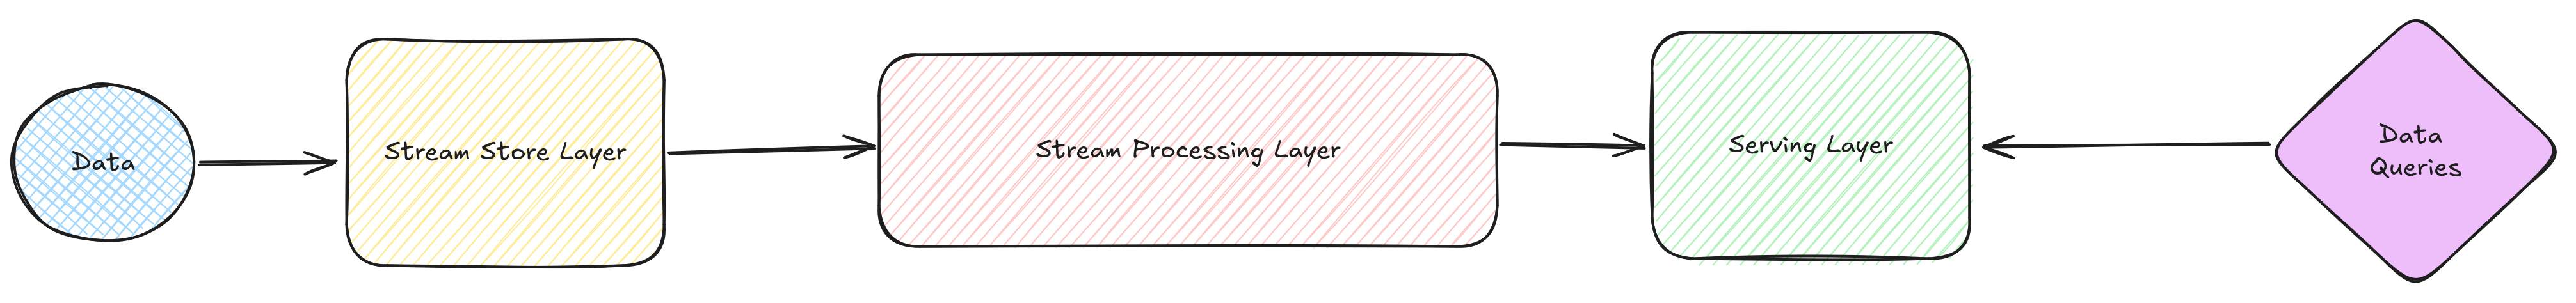
\includegraphics[width=0.8\textwidth]{teorico/kappa.png}
\caption{Diagrama de la Arquitectura Kappa}
\label{fig:arquitectura_kappa}
\end{figure}

\subsubsection{Implementación Típica}
\begin{figure}[h]
\centering
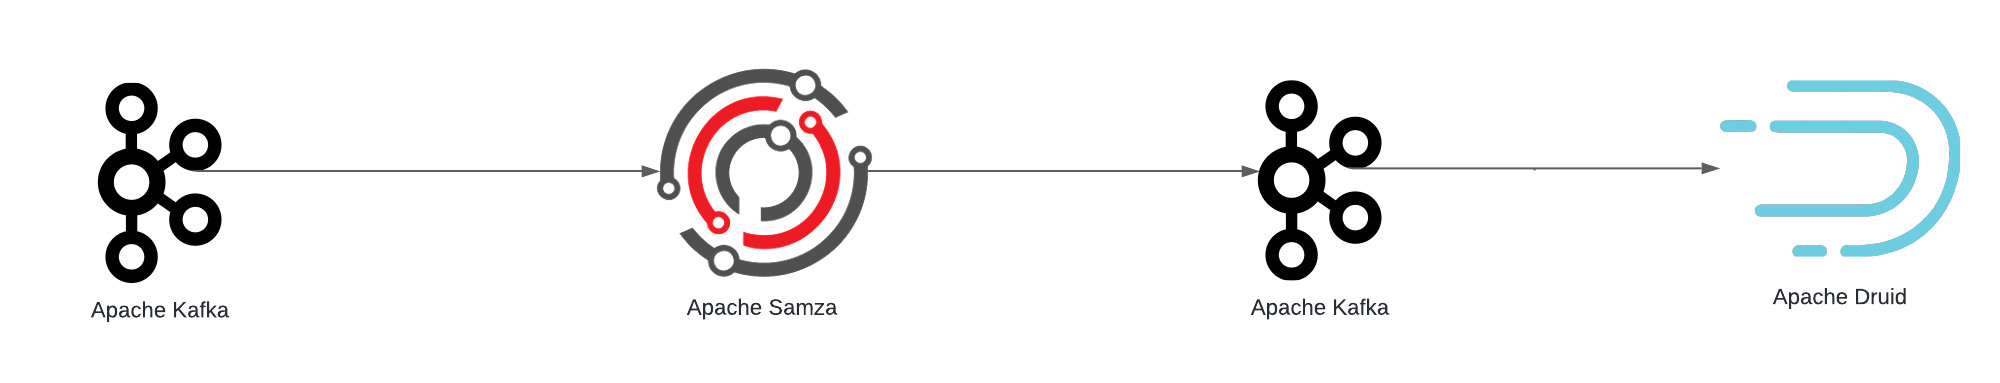
\includegraphics[width=0.8\textwidth]{teorico/KappaImplement.png}
\caption{Implementacion de la Arquitectura Kappa}
\label{fig:implementation_arquitectura_kappa}
\end{figure}

\subsection{Capacidades}
La Arquitectura Kappa ofrece varias capacidades clave:
\begin{itemize}
    \item \textbf{Simplificación}: Al unificar el procesamiento batch y en tiempo real, reduce la complejidad del sistema.
    \item \textbf{Consistencia}: Garantiza la coherencia entre los resultados del procesamiento en tiempo real y el reprocesamiento.
    \item \textbf{Reprocesamiento}: Permite actualizaciones de forma relativamente simple de la lógica de procesamiento mediante el reprocesamiento del stream.
\end{itemize}

\subsection{Desafíos}
A pesar de sus ventajas, la Arquitectura Kappa presenta algunos desafíos:
\begin{itemize}
    \item \textbf{Complejidad tecnologica}: Requiere tecnologias con caracteristicas muy especificas en la capa de Stream Store.
    \item \textbf{Recursos}: Requiere un incremento en el uso de recursos muy grande cuando es necesario reprocesar los datos históricos.
    \item \textbf{Complejidad}: Algunos análisis complejos pueden ser más difíciles de implementar en un modelo puramente basado en Streams.
\end{itemize}

\subsection{Conclusiones}
La Arquitectura Kappa representa una alternativa interesante en el diseño de sistemas de procesamiento de datos, 
ofreciendo una solución elegante para unificar el procesamiento batch y en tiempo real. 
Su enfoque en el procesamiento de streams como paradigma único simplifica la arquitectura general y reduce la complejidad del mantenimiento del código.
\newpage
\section{Arquitectura Delta}


La Arquitectura Delta surge desde Databricks, al igual que la Arquitectura Kappa, 
como una respuesta a los desafíos que presenta la arquitectura Lambda.
A diferencia de la suposición que hace Kappa de que todo puede ser tratado como un Stream, 
Delta por su parte, utiliza el almacenamiento de objetos en la nube como sustrato de almacenamiento y 
agrega por encima tecnología de metadata que otorga la posibilidad de utilizar este sistema de almacenamiento
como un canal de mensajes de modo que se puede hacer Streaming sobre él; además de agregar otras capacidades.
Esto permite utilizar una única tecnología tanto para análisis en tiempo real como análisis histórico. 


\subsection{Fundamentos y principios de diseño}

Delta parte de la premisa de que es deseable separar la capacidad de cómputo de la capacidad de almacenamiento; 
y que además es deseable hacerlo en base a sistemas de almacenamiento de objetos en la nube ya que son extremadamente
baratos y escalables. 

El desafío es entonces, alcanzar un almacenamiento que tenga buen rendimiento y que permita ser mutable sobre
este tipo de sistemas. Como se describió previamente, estos sistemas de almacenamiento tienen dificultades
en cuanto a la correctitud y el rendimiento en cuanto se intentan mutar multiples objetos a la vez. Un ejemplo
podría ser, la actualización del dataset entero para un usuario por cuestiones de normativa como GDPR.

La solución a este tipo de problemas, es un formato de tabla analítica sobre el almacenamiento subyacente. 


\subsubsection{Formato de Tabla Analítica}

Los formatos de tabla analítica son tecnologías diseñadas para resolver los desafíos del manejo de datos
a gran escala. Surgen como respuesta a las limitaciones de los formatos de archivo tradicionales como Parquet y ORC
cuando se trabaja con ellos en la nube. 

Las características más importantes que aporta un formato de tabla analítica son:
\begin{itemize}
    \item Soporte para transacciones ACID
    \item Control de versiones en los datos
    \item Capacidad de realizar operaciones de actualización y eliminación múltiples
    \item Compatibilidad con múltiples motores de procesamiento
\end{itemize}

Los formatos de tablas analíticas dan a sus sistemas subyacentes estas características a través de diferentes mecanismos y estrategias. 
La principal es la gestión de metadatos, ya que implementan estructuras de datos altamente optimizadas que permiten rastrear 
eficientemente los archivos y sus cambios; mientras mantienen un historial detallado de transacciones que garantiza la consistencia de los datos, 
complementando con estrategias efectivas de particionamiento y organización. 

Para la optimización del rendimiento, estos formatos emplean diversas técnicas como la compactación automática de archivos, 
estrategias de caching de datos para acceso rápido, utilización de formatos de archivo columnares como Parquet u ORC, 
y la incorporación de capacidades avanzadas de indexación y filtrado optimizado. 
La consistencia de los datos se garantiza mediante la implementación de transacciones ACID completas, 
que proporcionan un sólido aislamiento entre operaciones de lectura y escritura, manejan conflictos de manera automática 
y aseguran la consistencia en escenarios de operaciones concurrentes. 
En cuanto a la evolución y mantenimiento, estos formatos facilitan cambios de esquema sin interrupciones en el servicio. 

Todas estas mecanismos trabajan en conjunto para proporcionar una solución completa para el manejo de datos a escala masiva,
que como subproducto permite tratar la escritura de los archivos como un canal de mensajes sobre el que se puede hacer streaming.

Los exponentes más importantes de estos formatos son: Delta Table, Apache Iceberg y Apache Hudi


\subsubsection{Delta Lake}

Delta Lake (diseñada por Databricks) implementa una arquitectura de almacenamiento que se construye sobre archivos Parquet como formato base, 
organizándolos en una estructura de directorios. 
Cada tabla Delta está compuesta por dos elementos fundamentales: los archivos de datos en formato Parquet y el directorio {\_delta\_log} 
que contiene los metadatos y el registro de transacciones. 
Esta estructura permite mantener las ventajas de rendimiento y compresión eficiente de Parquet 
mientras añade capacidades transaccionales y de control de versiones.

El {\_delta\_log} representa el componente central que permite mantener el control de versiones y garantizar las propiedades ACID. 
Funciona como un registro detallado de cambios donde cada modificación se almacena en archivos JSON numerados secuencialmente. 
Cada uno de estos archivos contiene una o más acciones como añadir o eliminar archivos, actualizar metadatos, entre otras operaciones. 
Las transacciones se registran de forma atómica mediante operaciones del sistema de archivos, 
permitiendo reconstruir el estado exacto de la tabla en cualquier momento consultando este historial de cambios.

Para optimizar el rendimiento, se implementa un sistema de checkpoints que se generan automáticamente 
cada cierto número de transacciones. 
Estos checkpoints contienen una imagen completa del estado de la tabla en formato Parquet, 
evitando la necesidad de procesar todo el log desde el inicio al leer la tabla. 
Incluyen información crucial como la lista de archivos válidos, el esquema actual, la configuración de particionamiento 
y estadísticas detalladas de la tabla, funcionando como puntos de referencia rápidos para acceder al estado de la tabla.

El manejo de concurrencia se realiza a través de un sistema que combina control de concurrencia optimista con serialización de escrituras. 
Este enfoque permite que múltiples lectores y escritores trabajen simultáneamente mientras mantiene la consistencia de los datos. 
Las lecturas operan bajo "snapshot isolation", garantizando que cada lector vea una versión consistente de los datos,
mientras que las escrituras se serializan mediante un protocolo no bloqueante 
que utiliza operaciones atómicas del sistema de archivos para coordinación. 
El sistema incluye lógica de reintento automático para manejar conflictos de manera elegante.

Las características principales de Delta Lake incluyen transacciones ACID completas que garantizan consistencia en todas las operaciones, 
capacidades de acceder a versiones anteriores de los datos y volver atrás cuando sea necesario, 
y un sistema de evolución de esquema que previene la corrupción de datos. 
Las operaciones de Merge (UPSERTS) son particularmente sofisticadas, 
permitiendo actualizaciones eficientes de registros existentes con soporte para operaciones incrementales y condiciones de merge personalizables.

La optimización de datos es automática y tiene múltiples mecanismos, 
incluyendo compactación de archivos pequeños, optimización de consultas, y mantenimiento de estadísticas detalladas 
para mejor planificación de consultas. 

El soporte para streaming proporciona procesamiento de datos en tiempo real con semántica exactly-once y control de carga.

También presenta una excelente integración con Spark, aunque no tanto otros motores de procesamiento.

\subsubsection{Apache Hudi}

Apache Hudi (diseñado incialmente por Uber) implementa un sistema de almacenamiento que ofrece dos tipos principales de tablas: 
Copy On Write (COW) y Merge On Read (MOR). 
Las tablas COW almacenan datos directamente en formato columnar Parquet, donde cada actualización genera nuevas versiones de los archivos completos, 
optimizando así las lecturas pero con un mayor costo en escrituras.
Por otro lado, las tablas MOR utilizan un enfoque híbrido que combina archivos base en formato Parquet con archivos delta en formato Avro 
para los cambios recientes, proporcionando un balance entre rendimiento de lectura y escritura.

La gestión de metadatos se realiza mediante una Timeline que registra cronológicamente todas las acciones en una tabla. 
Estas incluyen COMMIT para nuevas inserciones o actualizaciones, {DELTA\_COMMIT} para escrituras en archivos delta en tablas MOR, 
CLEAN para limpieza de versiones antiguas, COMPACTION para la fusión de archivos delta con archivos base, RESTORE para rollbacks 
y SAVEPOINT para marcar puntos de recuperación específicos. 
Cada acción en la Timeline tiene un instant time único y mantiene metadatos detallados que permiten reconstruir el estado de la tabla 
en cualquier momento.

Para optimizar las operaciones, Hudi implementa un sistema de indexación versátil que incluye diferentes tipos de índices 
para búsquedas rápidas y la posibilidad de implementar índices personalizados. 
Esto facilita la localización eficiente de registros, optimiza las operaciones de upsert, 
maneja la deduplicación de datos y permite un ruteo optimizado de las escrituras.

Las características principales de Hudi incluyen un sistema de procesamiento incremental que permite manejar streams de datos incrementales, 
junto con consultas incrementales eficientes. 
El control de concurrencia se maneja a través de un control de concurrencia optimista que mantiene las lecturas sin bloqueos mientras 
serializa las escrituras para mantener la consistencia. 
Además, Hudi implementa características como gestión de compactación automática configurable, 
y un sistema de limpieza que mantiene el almacenamiento optimizado.

El manejo de registros individuales en Hudi es particularmente sofisticado, ofreciendo versionado a nivel de registro, borrado lógico, 
evolución de esquemas y actualizaciones a nivel de fila. 
Todo esto se mantiene bajo fuertes garantías de consistencia que incluyen transacciones ACID y semántica exactly-once. 

También presenta una muy buena integración con diferentes motores de procesamiento como Spark y Flink.

\subsubsection{Apache Iceberg}

Apache Iceberg (diseñado inicialmente por Netflix) implementa una arquitectura de almacenamiento que se distingue por su 
modelo de metadatos y su enfoque en la evolución del esquema. 
El formato utiliza una estructura de tabla que separa completamente los metadatos de los datos, 
manteniendo varios niveles de manifiestos que rastrean todos los archivos de datos. 
Esta jerarquía de metadatos incluye un archivo de metadatos principal, manifest lists que agrupan archivos de manifiesto, 
y manifiestos individuales que rastrean los archivos de datos. 
Los datos en sí se almacenan en formatos como Parquet o ORC, permitiendo una optimización efectiva para consultas analíticas.

El sistema de control de versiones de Iceberg se implementa a través de un modelo de snapshots atómicos. 
Cada snapshot representa un punto en el tiempo inmutable de la tabla y contiene referencias a todos los archivos de datos válidos para esa versión. 
Los snapshots se encadenan entre sí, formando un historial lineal de la tabla, permitiendo ir hacia atrás en el tiempo. 
Este diseño facilita las operaciones concurrentes y garantiza la consistencia sin necesidad de bloqueos pesados, 
ya que cada operación de escritura crea un nuevo snapshot sin modificar los existentes.

La gestión de esquemas en Iceberg permite evolucionar tanto el esquema de la tabla como la estrategia de particionamiento 
sin necesidad de reescribir datos. 
El sistema mantiene un historial de esquemas y asigna identificadores únicos a cada campo, 
permitiendo cambios seguros como añadir, renombrar o reordenar columnas. 
El particionamiento es tratado como metadatos, lo que permite cambiar la estrategia de particionamiento sin mover datos, 
una característica única que facilita la optimización continua del rendimiento de las consultas.

La optimización de consultas en Iceberg se beneficia de su capa de metadatos. 
El formato mantiene estadísticas detalladas a nivel de columna y archivos, 
incluyendo valores mínimos y máximos, conteos de nulos y otros metadatos que permiten una poda eficiente de particiones 
y archivos durante la planificación de consultas. A
demás, implementa características como la posibilidad de realizar lecturas incrementales eficientes, 
filtrado de datos a nivel de manifiesto, y soporte para operaciones de reescritura de datos optimizadas.

El control de concurrencia en Iceberg utiliza un enfoque optimista basado en la inmutabilidad de los snapshots. 
Las operaciones de lectura siempre ven una vista consistente de la tabla basada en un snapshot específico, 
mientras que las escrituras compiten por crear el siguiente snapshot en la cadena. 
Los conflictos se detectan y resuelven al momento del commit, y el sistema proporciona garantías de aislamiento y consistencia 
sin requerir un sistema de bloqueo centralizado.

Las características de mantenimiento incluyen la expiración de snapshots antiguos, compactación de archivos pequeños, 
y reescritura de datos para optimización física. 
Estas operaciones se pueden realizar de manera concurrente con las operaciones normales de lectura y escritura.

La integración con diferentes motores de procesamiento es otro punto fuerte ya que proporciona APIs nativas para Spark, Flink, y otros motores, 
permitiendo que cada motor optimice su acceso aprovechando las características avanzadas de metadatos y estadísticas.

\subsection{Vista Lógica}



\subsection{Implementación Típica}

\subsection{Ventajas}

\subsection{Desafíos}



\subsection{Casos de uso ideales}

\chapter{Metodología}


\section{Criterios de Evaluación}

Para evaluar y comparar las arquitecturas Kappa y Delta en el contexto del monitoreo remoto de pacientes, se considerarán creiterios unificados y medibles.
Estos servirán como base para una evaluación objetiva de las arquitecturas Kappa y Delta en el contexto del monitoreo remoto de pacientes, permitiendo tomar criterios 
fundamentados para la elección de una u otra según el escenario.

\newpage

\subsection{Latencia y Rendimiento}

Se implementarán mediciones a través de puntos de instrumentación estratégicos a lo largo de los componentes de la arquitectura.  
Estos puntos de medición incluirían timestamps en los mensajes, métricas de procesamiento en los componentes intermedios, y el tiempo de escritura/lectura en la capa final. 

Las métricas serán tomadas utilizando Prometheus y mostradas en un tablero de Grafana.

Las métricas a considerar serán:
\begin{itemize}
    \item Tiempo de ingesta de histórico
    \item Latencia de procesamiento
\end{itemize}

\subsection{Manejo de Datos Históricos}

Se medirán especificamente la efectividad con la que el sistema permite consultar datos históricos y reprocesar toda la historia.
Las métricas serán tomadas utilizando Prometheus y mostradas en un tablero de Grafana.

\begin{itemize}
    \item Tiempo de reprocesamiento de la historia completa
    \item Uso de recursos en reprocesamiento de la historia completa
\end{itemize}

Se omitirá la implementación de un cambio en el modelo de procesamiento que implique reprocesar la historia completa, 
pero se dará una propuesta de como hacerlo y se evaluará las implicancias de su puesta en producción manteniendo los dos sistemas funcionando e integrandolos eventualmente.

\subsection{Costos Operativos}

La implementación del sistema en contenedores, permitirá un monitoreo del uso de los recursos del sistema.
Además, se plantearán cálculos, utilizando las calculadoras de costo que proveen los sistemas de nube, que permitan dimensionar el costo operativo de estos sistemas.
Las métricas serán tomadas utilizando Prometheus y mostradas en un tablero de Grafana.

Las métricas a considerar serán:
\begin{itemize}
    \item Uso de memoria RAM
    \item Uso de CPU
    \item Uso de disco
    \item Uso de red
\end{itemize}

\newpage
\section{Stack de Tecnologías a Utilizar}

Con el objetivo de comparar objetivamente las arquitecturas Kappa y Delta, 
se definió un stack tecnológico común que permite mantener condiciones similares en términos de despliegue, 
monitoreo y operación.\newline 

Estas tecnologías fueron seleccionado considerando aspectos como compatibilidad, 
madurez del ecosistema, integración con otras herramientas, facilidad de operación, 
disponibilidad de documentación y eficiencia de recursos.

\subsection*{Sistema de Mensajería - Apache Kafka}

Apache Kafka fue elegido como el punto de entrada del sistema por ser el estándar de facto en mensajería distribuida en arquitecturas de datos modernas. 
Su arquitectura distribuida permite alta disponibilidad, tolerancia a fallos, retención configurable 
y orden garantizado en particiones. \newline

Kafka desacopla la ingesta del procesamiento, permitiendo escalabilidad horizontal 
y resiliencia ante picos de carga.\newline

Se hicieron pruebas con Apache Pulsar, que promete ser el sucesor de Kafka,
pero su adopción en la industria es aún limitada y su ecosistema de herramientas no es tan maduro.
A su vez, su documentación presenta inconsistencias que hacen un desafío su integración en escenarios poco convencionales. \newline

\newpage

\subsection*{Motor de Procesamiento de Flujos - Apache Flink}

Flink fue seleccionado por su baja latencia, manejo avanzado de estado y compatibilidad directa con fuentes como Kafka y formatos de tablas analíticas como Apache Paimon.\newline 

Su modelo de programación basado en flujos de datos y su integración con catálogos lo hacen ideal tanto para arquitecturas Kappa como Delta.\newline 

Además, permite operaciones con garantías \textit{exactly-once} y es capaz de reprocesar eventos desde el principio del log si fuera necesario.\newline

Aunque Apache Spark Structured Streaming podría haber sido considerado, 
Flink presenta menor latencia y mejor soporte para semánticas de estado complejas.

\subsection*{Almacenamiento de Objetos - MinIO}

MinIO fue elegido como la solución de almacenamiento distribuido compatible con la API de S3. 
Su facilidad de despliegue, rendimiento eficiente y compatibilidad con entornos locales lo posicionan como una alternativa ideal a soluciones propietarias en la nube, 
permitiendo independencia de proveedor y bajo costo operativo.

\subsection*{Formato de Tabla Analítica - Apache Paimon}

Apache Paimon fue seleccionado como formato de tabla debido a su diseño nativo para flujos de datos. 
Su integración con Flink es directa y permite operaciones de escritura eficientes en escenarios de actualización frecuente. 
A pesar de tener una comunidad pequeña, 
su especialización para el procesamiento incremental en tiempo real fue clave para esta elección.\newline

Otras alternativas como Apache Iceberg o Hudi tienen comunidades más grandes y mejor documentación, 
pero presentan mayores desafíos en integración directa con Flink 
o no funcionan también para el caso de procesamiento de streaming.

\newpage

\subsection*{Motor Analítico - Apache Doris}

Doris combina procesamiento paralelo masivo (MPP) con consultas OLAP en tiempo real. 
Su soporte para tablas híbridas y la posibilidad de realizar consultas federadas sin necesidad de duplicar los datos lo convierte en una excelente opción para analítica en tiempo real e histórica.
También la integración con Paimon mediante un catálogo lo posiciona como una solución eficiente y simple de operar.\newline

Aunque Druid o Pinot fueron considerados, 
Doris ofrece capacidades que estas otras tecnologías no tienen. En particular, las consultas federadas.

\subsection*{Orquestación de Contenedores - Docker Compose}

El uso de Docker Compose permite una gestión simple, portable y reproducible del entorno experimental. 
Facilita el aislamiento de componentes, el control de versiones de imágenes y la replicabilidad del experimento. \newline

Esta elección responde a la necesidad de contar con un entorno controlado sin la complejidad que presentan otras herramientas.

\subsection*{Monitoreo y Visualización: Prometheus + Grafana}

Prometheus permite recolección y análisis eficiente de métricas, 
mientras que Grafana proporciona una interfaz amigable y personalizable para visualizar el estado del sistema y comparar el rendimiento entre arquitecturas. 

Esta combinación es ampliamente adoptada en entornos productivos, y su integración nativa con sistemas de contenedores y servicios distribuidos la vuelve especialmente útil para este caso.

Además, se aprovecha la capacidad de Grafana para crear paneles de control personalizados 
para también visualizar los resultados de las consultas analíticas.

\newpage
\section{Despliegue}

Se realizará un despliegue de ambas arquitecturas manteniendo la misma cantidad de nodos de cada tecnología.
Para esto se utilizarán contenedores con la tecnología Docker Compose dentro de una única máquina virtual linux.
El sistema donde se desplegará el sistema cuenta con 16 núcleos, 64 GB de RAM y 2 TB de disco duro de estado sólido.
El sistema operativo utilizado es Ubuntu 22.04 LTS.

\subsection{Componentes}

Se desplegarán los siguientes componentes: 

\begin{longtable}{|p{6cm}|p{6cm}|}
    \hline
    \textbf{Componente} & \textbf{Cantidad} \\
    \hline
    \endhead
    Broker Apache Kafka & 3 \\ 
    \hline
    Zookeeper & 3 \\ 
    \hline
    Apache Flink Job Manager & 1 \\ 
    \hline
    Apache Flink Task Manager & 4 \\ 
    \hline
    Apache Doris Frontend & 1 \\ 
    \hline
    Apache Doris Backend & 3 \\ 
    \hline
    MinIO & 1 \\ 
    \hline
    Grafana & 1 \\ 
    \hline
    Prometheus & 1 \\ 
    \hline 
    \caption{Cantidad de componentes desplegados}
    \label{tab:deployed_components}
\end{longtable}

El objetivo de esta configuración es proveer de un entorno de alta disponibilidad que a su vez permita escalar horizontalmente y
se adecúe al ambiente de pruebas.

\newpage

\subsection{Configuración de los componentes}

Se utilizarán configuraciones por defecto para cada uno de los componentes desplegados.
Sin embargo, se realizán los cambios necesarios para asegurar el correcto funcionamiento de los mismos.
Se deberá asegurar la mayor cantidad de recursos del sistema para cada uno de los componentes,
dándole mayor importancia a los componentes que se encargan de la ingestión y procesamiento de datos.
De esta forma, se deberá asegurar el procesamiento ininterrumpido de los datos.
\section{Mediciones}

Se realizarán mediciones de rendimiento y latencia de ambas arquitecturas.
Para esto se tomarán 5 muestras de cada medición y se calculará el promedio y la desviación estándar.
Las mediciones se realizarán en el mismo entorno de despliegue y con la misma carga de trabajo.
Se utilizará un conjunto de datos sintético que corresponden a 1 año de datos de 32 pacientes,
lo que implica alrededor de 7 GB de datos. 
Todas las mediciones se harán sobre un entorno recien instalado para asegurar que no haya interferencias entre mediciones.
Se desarrollará un script en Python que se encargará de enviar las mediciones a cada uno de los sistemas.
El script se encargará de enviar los datos a través de un productor de Kafka y lo hará tan rápido como sea posible,
lo que permitirá medir el impacto que tiene el despliege del sistema en el entorno donde se ejecuta.

\newpage
\section{Conjunto de Datos}

El conjunto de datos utilizado para evaluar el sistema será de datos sintéticos. 
Se desarrollará un script en Python que genere datos sintéticos para los sensores de signos vitales.\newline

Estos datos serán generados de acuerdo a la naturaleza de la medición de cada sensor y se interconectarán para simular un flujo de datos continuo.
El script generará datos para tres tipos de pacientes: Sanos, Sanos pero que se deterioran con el tiempo, y enfermos pero estables. 
De esta manera, se podrá evaluar el sistema en diferentes escenarios.\newline

Existen dos razones principales para el uso de datos sintéticos: 

\begin{itemize}
    \item Los conjuntos de datos de sensores disponibles son heterogéneos y muy pequeños; lo que de todos modos implicaría generar datos sintéticos
    \item No es necesario contar con datos que muestren tendencias reales, sino que se comporten como lo harían en realidad para demostrar los atributos de calidad del sistema
\end{itemize}

Para esto, se definirá un flujo de datos para cada sensor que será interconectado pero definiendo comportamientos especificos que tengan que ver con la naturaleza de su medición.
Los signos vitales tomados para esto son: 

\begin{itemize}
    \item Frecuencia respiratoria
    \item Presión sistólica
    \item Frecuencia cardíaca
    \item Temperatura
    \item Saturación de oxígeno
    \item Nivel de conciencia en escala APVU
\end{itemize}
\chapter{Desarrollo}

\section{Aclaraciones}

El desarrollo fué realizado a lo largo de 9 meses de trabajo, y todos los avances fueron subidos a repositorios privados de GitHub.
Para mejorar la transparencia en el proceso de desarrollo y monitorear avances estos repositorios se hicieron públicos.
De esta forma, se pueden ver los cambios hechos en cada momento del desarrollo.
\newpage
\section{Monitoreo Remoto de Pacientes}

\subsection{Introducción}

\subsubsection{Antecedentes}
El Monitoreo Remoto de Pacientes ha emergido como una tecnología para mejorar la atención médica moderna, permitiendo la vigilancia continua del paciente fuera de los entornos clínicos tradicionales. 
Sin embargo, estos sistemas enfrentan desafíos en el mantenimiento de la calidad consistente de datos y la integración de mediciones de múltiples dispositivos con diferentes niveles de confiabilidad 
y tasas de muestreo.

\subsubsection{Planteamiento del Problema}
Los sistemas tradicionales de monitoreo de signos vitales frecuentemente enfrentan dificultades con:
\begin{itemize}
    \item Temporización inconsistente de mediciones entre diferentes signos vitales
    \item Variación en la confiabilidad y precisión de los dispositivos
    \item Integración de múltiples fuentes de datos para el mismo signo vital
    \item Mantenimiento de la validez clínica con datos incompletos
\end{itemize}

\newpage
\subsubsection{Solución Propuesta}
Se propone abordar estos desafíos mediante:
\begin{itemize}
    \item Fusión de datos multi-dispositivo 
    \item Puntaje de calidad del dato
    \item Puntaje de frescura del dato
    \item Capacidad de degradación gradual
\end{itemize}

\subsection{Sistema de Puntuación NEWS2}

\subsubsection{Descripción General de NEWS2}
El National Early Warning Score 2 (NEWS2) es una herramienta de evaluación estandarizada utilizada para detectar el deterioro clínico. Evalúa seis parámetros fisiológicos:
\begin{itemize}
    \item Frecuencia respiratoria
    \item Saturación de oxígeno
    \item Presión arterial sistólica
    \item Frecuencia cardíaca
    \item Nivel de consciencia
    \item Temperatura
\end{itemize}

\subsubsection{Desafíos de Implementación Tradicional}
NEWS2 fue originalmente diseñado para mediciones manuales periódicas en entornos clínicos. Su adaptación para monitoreo remoto continuo presenta varios desafíos:
\begin{itemize}
    \item Diferentes frecuencias de medición para diferentes parámetros
    \item Calidad y confiabilidad variable de las mediciones
    \item Necesidad de actualizaciones de puntuación en tiempo real
    \item Manejo de datos faltantes o degradados
\end{itemize}

\subsection{gdNEWS2}

\subsubsection{Concepto y Fundamentos}
Se propone aumentar el sistema NEWS2 con el concepto de degradación gradual (graceful degradation) de modo que la puntuación aún sea útil incluso cuando la medición de alguno de los datos de signos vitales no 
se encuentre presente o no se confíe del todo en la calidad del mismo.\newline

Cada parámetro de NEWS2 tiene un puntaje de calidad y de frescura asociado, que se utilizarán para definir el nivel de confianza que se le tiene a dicho parámetro.
De esta forma, se puede calcular una puntuación de alerta temprana incluso cuando no se tienen todos los datos disponibles 
y brindarle transparencia al profesional de la salud para que tome las decisiones correspondientes en cuanto al tratamiento del paciente.

\subsection{Formato de Datos de Mediciones Brutas}

Los datos serán recibidos en formato JSON, con un esquema común para todos los tipos de mediciones.
El esquema general es el siguiente:
\begin{lstlisting}[
    frame=single,
    numbers=left,
    numbersep=5pt,
    xleftmargin=20pt,
    language=JSON,
    basicstyle=\ttfamily,
    commentstyle=\color{gray},
    caption={JSON example},
    label={json-example}]
{
    "measurement_type": "RESPIRATORY_RATE" | "HEART_RATE" | "OXYGEN_SATURATION" | "BLOOD_PRESSURE_SYSTOLIC" | "TEMPERATURE" | "CONSCIOUSNESS",
    "measurement_timestamp": "datetime",
    "device_id": "string",
    "raw_value": "number",
    "battery": "number",
    "signal_strength": "number"
}
\end{lstlisting}
\newpage

\subsection{Algoritmo de Puntuación de Calidad}
Un nuevo algoritmo de puntuación de calidad debería basarse en la experiencia clínica y la evidencia científica. Para el caso de estudio presentado, 
se propone un algoritmo sencillo, a fin de ilustrar su potencial y mantener limitado el enfoque de este trabajo.\newline

Se tomarán los identificadores de los dispositivos, que luego serán clasificados en 3 grupos cada uno con un peso asociado: 

\begin{longtable}{|p{6cm}|p{3cm}|}
    \hline
    \textbf{Clasificación de Dispositivos} & \textbf{Peso Asociado} \\
    \hline
    \endhead
    Dispositivos de calidad médica & 1.0 \\
    \hline
    Dispositivos de calidad premium & 0.7 \\
    \hline
    Dispositivos de calidad de consumo & 0.4 \\
    \hline
    \caption{Clasificación de dispositivos y sus pesos correspondientes}
    \label{tab:dispositivos}
\end{longtable}

Además, se tomará en cuenta la señal de batería y la intensidad de la señal, que serán clasificados en 3 grupos cada uno con un peso asociado:

\begin{longtable}{|p{6cm}|p{3cm}|}
    \hline
    \textbf{Nivel de Batería} & \textbf{Peso Asociado} \\
    \hline
    \endhead
    Batería a más del 80\% & 1.0 \\
    \hline
    Batería entre 80\% y 50\% & 0.7 \\
    \hline
    Batería entre 50\% y 20\% & 0.6 \\
    \hline
    Batería a menos de 20\% & 0.4 \\
    \hline
    \caption{Clasificación de niveles de batería y sus pesos correspondientes}
    \label{tab:bateria}
\end{longtable}

Por último, se tomará en cuenta la intensidad de la señal:
\begin{longtable}{|p{6cm}|p{3cm}|}
    \hline
    \textbf{Intensidad de Señal} & \textbf{Peso Asociado} \\
    \hline
    \endhead
    Valor de señal de más de 0.8 & 1.0 \\
    \hline
    Valor de señal entre 0.8 y 0.6 & 0.8 \\
    \hline
    Valor de señal entre 0.5 y 0.6 & 0.6 \\
    \hline
    Valor de señal menor a 0.5 & 0.4 \\
    \hline
    \caption{Clasificación de intensidad de señal y sus pesos correspondientes}
    \label{tab:senal}
\end{longtable}

\newpage
De esta manera, el cálculo de la puntuación de calidad se realizará de la siguiente manera:


\begin{equation}
    \text{Quality Score} = 0.7 \times \text{Device Quality} + 0.2 \times \text{Battery Quality} + 0.1 \times \text{Signal Quality}
\end{equation}


En este momento, los valores tanto de los pesos como de los parámetros son arbitrarios y se espera que en caso de encontrar útil este acercamiento, 
futuras iteraciones ajusten estos parámetros o utilicen un criterio diferente para su cálculo.

\newpage

\subsection{Algoritmo de Puntuación de Frescura}

Para medir la frescura de los datos, se propone un enfoque simple que considera el tiempo transcurrido desde la última medición 
y el tiempo que le tomó a la medición actual llegar a ser procesada.\newline

Tiempo desde medición hasta procesamiento:
\begin{longtable}{|p{9cm}|p{3cm}|}
    \hline
    \textbf{Tiempo de Medición hasta Procesamiento} & \textbf{Peso Asociado} \\
    \hline
    \endhead
    Menos de una hora & 1.0 \\
    \hline
    Entre una y seis horas & 0.9 \\
    \hline
    Entre seis y doce horas & 0.7 \\
    \hline
    Entre doce y veinticuatro horas & 0.5 \\
    \hline
    Entre veinticuatro y cuarenta y ocho horas & 0.3 \\
    \hline
    Otros & 0.2 \\
    \hline
    \caption{Clasificación de tiempo desde medición hasta procesamiento}
\end{longtable}

Tiempos entre mediciones:
\begin{longtable}{|p{9cm}|p{3cm}|}
    \hline
    \textbf{Tiempo entre Mediciones} & \textbf{Peso Asociado} \\
    \hline
    \endhead
    Menos de cuatro horas & 1.0 \\
    \hline
    Entre cuatro y ocho horas & 0.8 \\
    \hline
    Entre ocho y doce horas & 0.6 \\
    \hline
    Entre doce y veinticuatro horas & 0.4 \\
    \hline
    Más de veinticuatro horas & 0.2 \\
    \hline
    \caption{Clasificación de tiempo entre mediciones}
\end{longtable}

De esta manera, se propone el siguiente algoritmo de puntuación de frescura:

\begin{equation}
    \text{Freshness Score} = 0.5 \times \text{Time Since Last Measurement} + 0.5 \times \text{Time Since Measurement}
\end{equation}

\newpage

\subsection{Algoritmo de Puntuación de Degradación}

Este algoritmo se encargará de calcular la puntuación de degradación de la puntuación NEWS2 en caso de que no se tengan todos los datos disponibles.
Simboliza la confianza que se le tiene a la puntuación NEWS2 en base a la calidad y frescura de los datos.\newline

Se propone utilizar la siguiente fórmula para calcular la puntuación de degradación:

\begin{equation}
    \text{Degradation Score} = 0.7 \times \text{Quality Score} + 0.3 \times \text{Freshness Score}
\end{equation}

Se calcula este puntaje para cada uno de los parámetros de NEWS2, y se promedia para obtener la puntuación de degradación final.

\subsection{Algoritmo de Puntuación de NEWS2}

El algoritmo de puntuación NEWS2 se basa en la suma de los puntajes de cada uno de los parámetros,
\begin{equation}
    \text{NEWS2 Score} = \sum_{i=1}^{n} \text{Parameter Score}_i
\end{equation}
donde $n$ es la cantidad de parámetros que se tienen disponibles.
En caso de que no se tenga un parámetro disponible, se asumirá una puntuación de cero para ese parámetro en su lugar.
De esta manera, se puede calcular la puntuación NEWS2 incluso cuando no se tienen todos los datos disponibles.\newline

Por otro lado, se propone utilizar la puntuación de degradación para dar contexto sobre la puntuación NEWS2 final.
Así, se puede explicar que tan confiable es la puntuación NEWS2 calculada en base a los datos disponibles.
\newpage
\section{Implementación}

Se implementará le especificación definida en el capítulo anterior de modo tal que para ambas arquitecturas los detalles de implementación sean lo más similares posible.
Para esto, se utilizará como lenguaje de procesamiento Flink SQL, que permite desarrollar los trabajos de procesamiento utilizando un lenguaje agnóstico a las plataformas subyascentes. 

\subsection{Pipeline de Procesamiento}
El pipeline de procesamiento se encargará de recibir los datos en formato JSON,
realizar el procesamiento de los mismos y devolver la puntuación NEWS2 calculada.

Esto se realizará de la siguiente manera:
\begin{itemize}
    \item Recepción de datos en formato JSON mediante un topico de Kafka
    \item Enriquecimiento de los datos con los puntajes de calidad y frescura
    \item Enrutamiento de los datos para su procesamiento particular según el signo vital
    \item Cálculo de la puntuación NEWS2 para cada una de las Componentes
    \item Unión y agrupación según una ventana de tiempo
    \item Calculo de valores de agregación de los puntajes de NEWS2 y de degradación
\end{itemize}

Debido a una limitante en el hardware de procesamiento, se simplificó el calculo de frescura de los datos para no tener en cuenta los anteriores. 
Esto provocaba que el sistema se quedara sin memoria y no pudiera procesar los datos para ambas arquitecturas. 
Por lo que se optó por no tener en cuenta los datos anteriores y solo calcular la frescura de los datos con las medidas de tiempo propias de cada registro.

A continuación se presenta un diagrama de flujo del pipeline de procesamiento:
\begin{figure}[h]
    \centering
    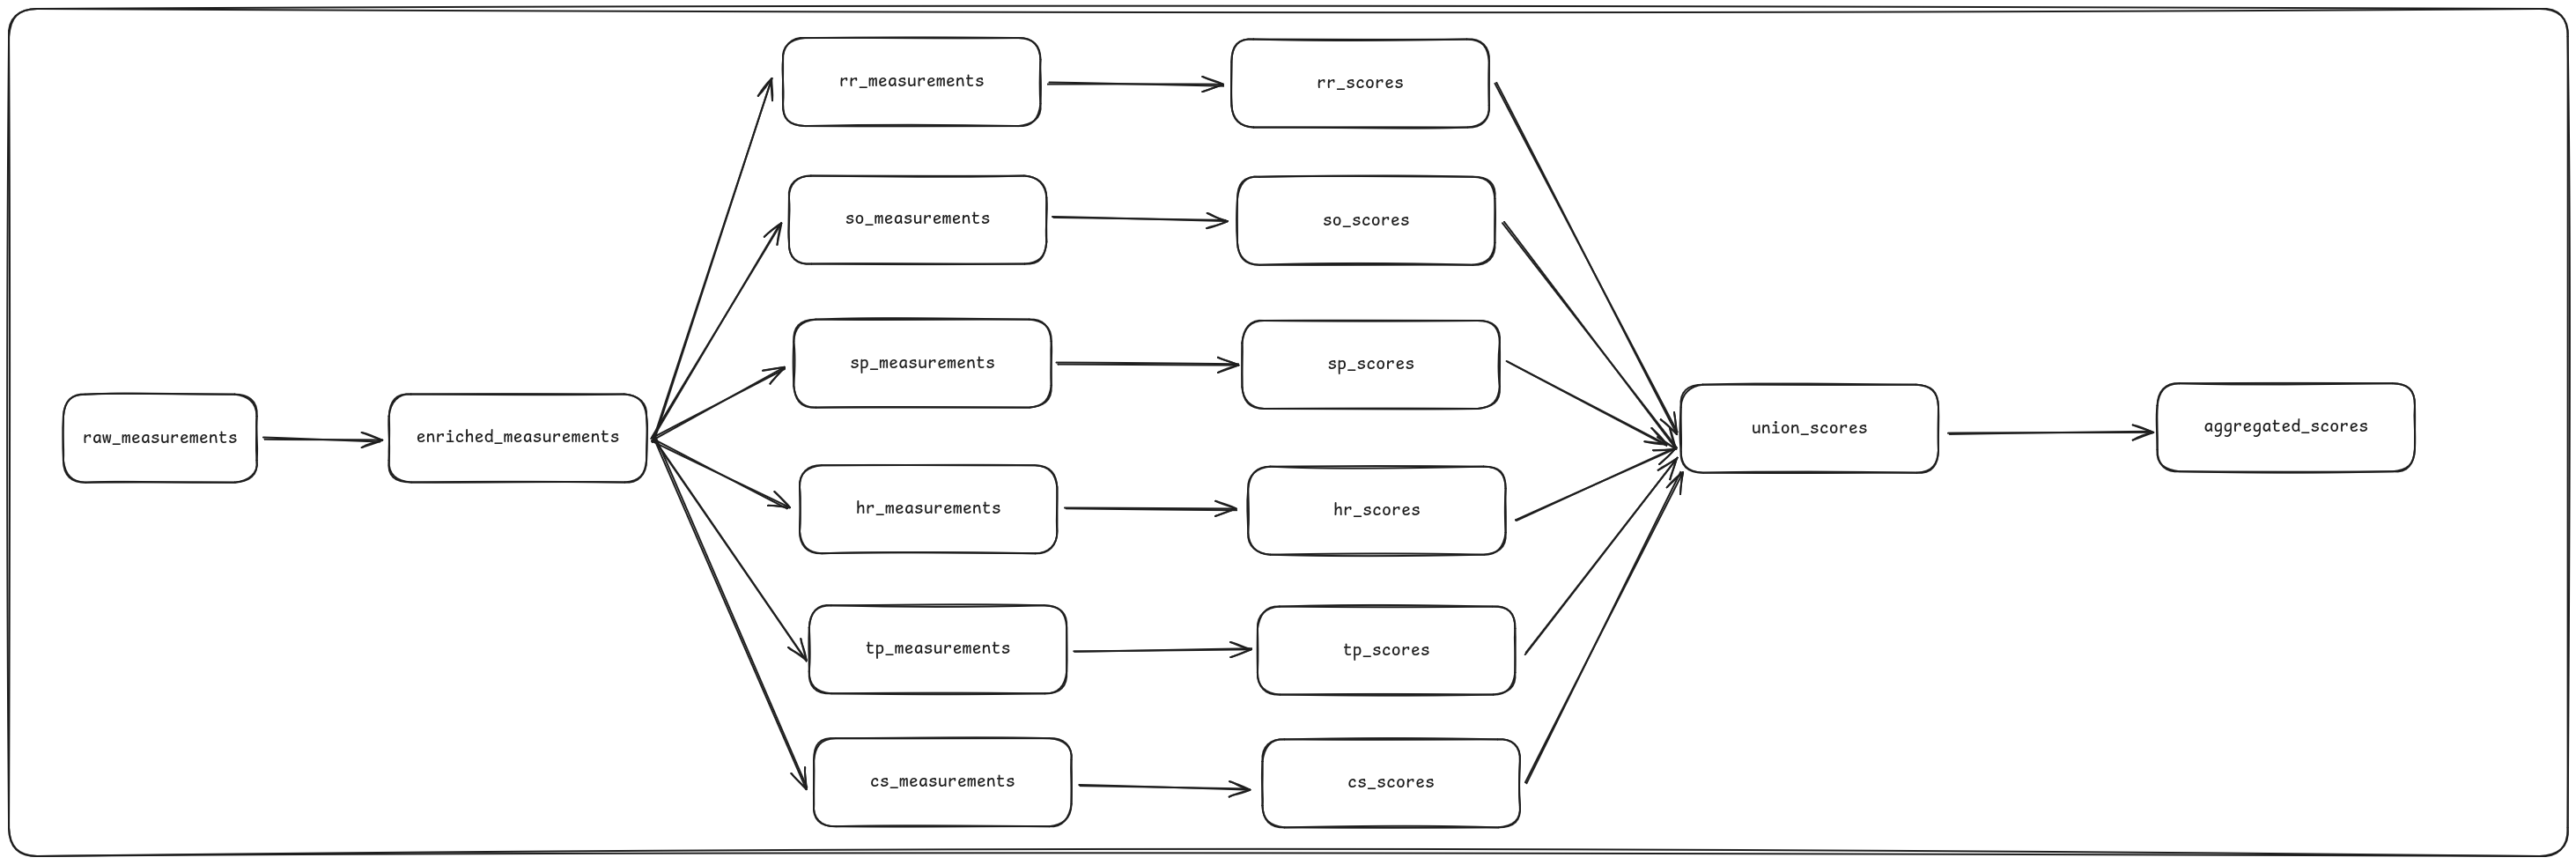
\includegraphics[width=1\textwidth]{desarrollo/pipeline.png}
    \caption{Diagrama de flujo del pipeline de procesamiento}
    \label{fig:flowchart}
\end{figure}

\clearpage

\subsection{Despliegue de Componentes}

El despliegue de los componentes se realizó mediante el uso de \textbf{Docker Compose}, y se midió según las métricas expuestas por esta herramienta.
Por otro lado, para el calculo de costos, se asume un despliegue de alta disponibilidad en la nube de AWS basado en el siguiente diagrama:

\begin{figure}[h]
    \centering
    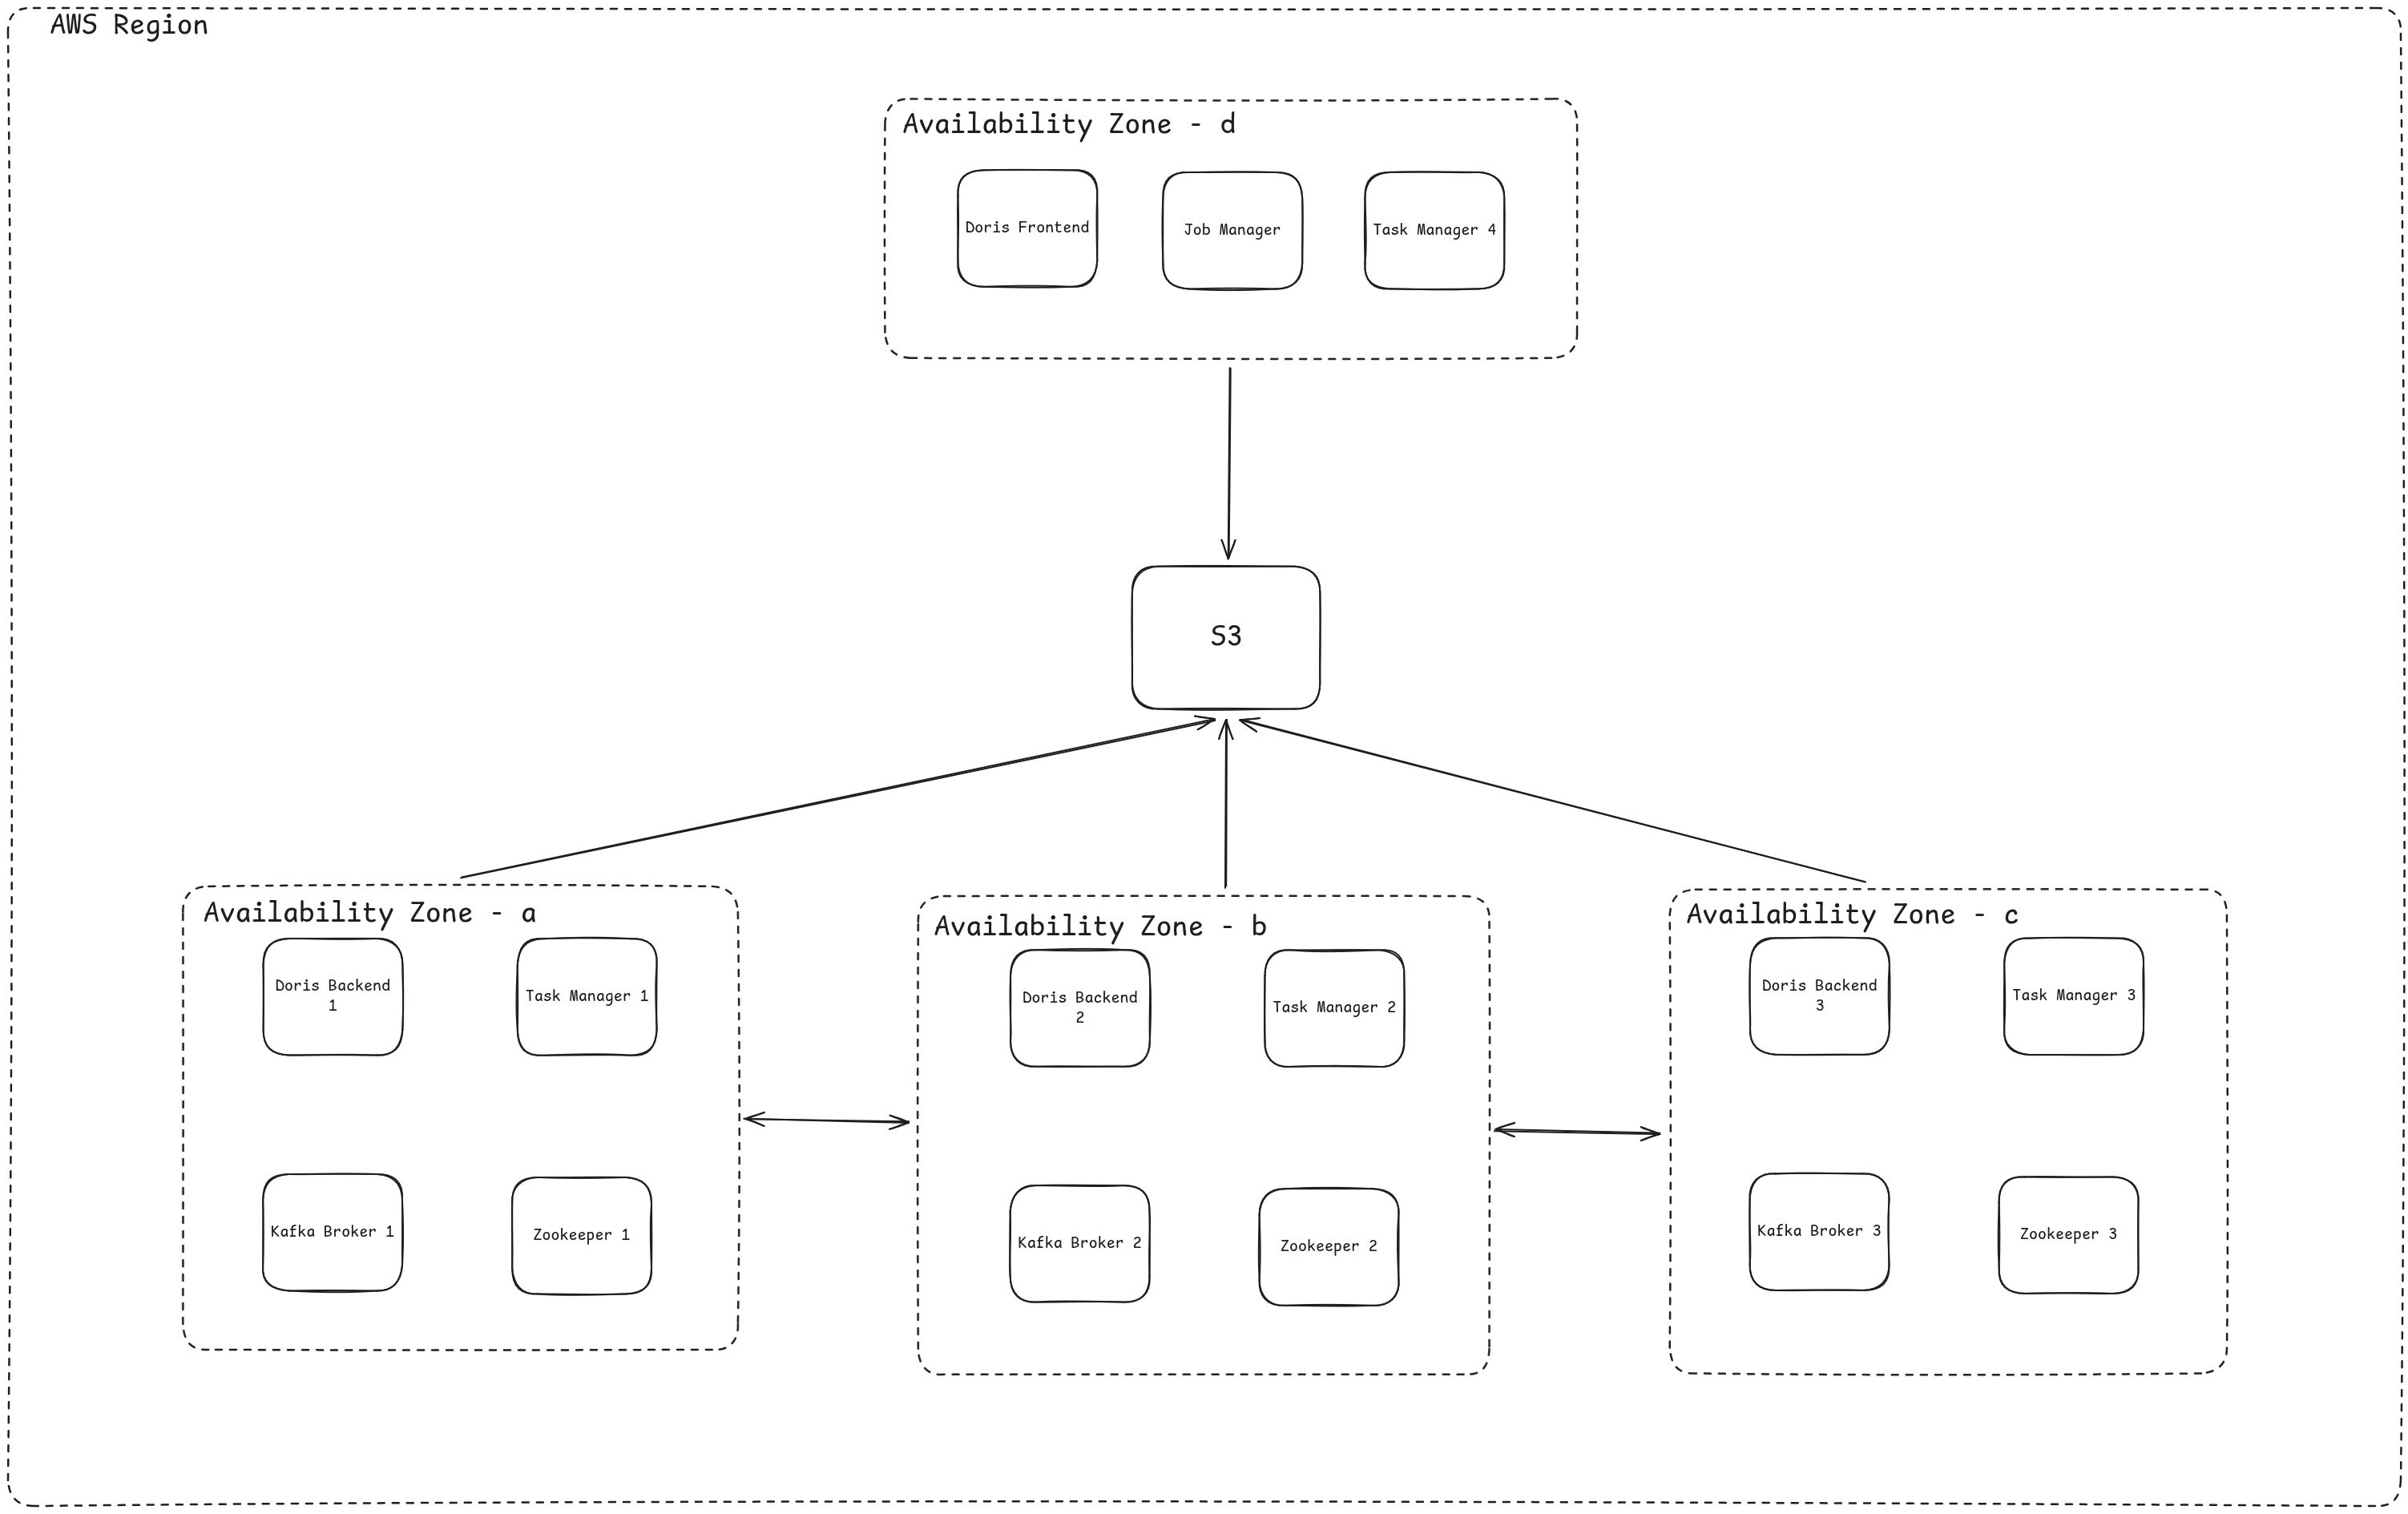
\includegraphics[width=1\textwidth]{desarrollo/deployment.png}
    \caption{Diagrama de despliegue de componentes}
    \label{fig:infraestructura}
\end{figure}

\clearpage

La razón de este despliegue es la alta disponibilidad y la tolerancia a fallos, por lo que se despliega en una única región 
y se dividen los servicios en zonas de disponibilidad para asegurar que si una de ellas falla,
el sistema siga funcionando lo mejor posible.

Tres de las zonas de disponibilidad (a, b y c) son idempotentes en cuanto a su funcionamiento, 
cada una cuenta con un nodo de Kafka, un nodo Zookeeper, un nodo de procesamiento de Flink y un nodo de backend de Doris.
La cuarta zona de disponibilidad (d) tiene el nodo de frontend de Doris y el nodo de gestión de Flink; así como también un nodo extra de procesamiento de Flink.
No se incluye MinIO en este despliegue porque se utiliza S3 nativo, que se define en una región y esta igualmente comunicado con todas las zonas de disponibilidad.

A su vez, estarían idealmente desplegados mediante un orquestador de contenedores como Kubernetes, utilizando algún servicio como Elastic Kubernetes Serice (EKS).


\subsection{Repositorio de Código}

Se definireron tres repositorios de código para el desarrollo de la arquitectura Kappa y Delta.
El primero de ellos es el repositorio de la arquitectura Kappa, que contiene el código de procesamiento de datos y la configuración de los componentes.
El segundo es el repositorio de la arquitectura Delta, que contiene el código de procesamiento de datos y la configuración de los componentes.
El tercero es el repositorio del generador de datos sintéticos que se utilizó para realizar las pruebas de carga y estrés.

El código de cada uno de los repositorios se encuentra disponible en el siguiente enlace:

\begin{itemize}
    \item \url{https://github.com/Rekeyea/Tesis-Kappa}\\
    \item \url{https://github.com/Rekeyea/Tesis-Delta}\\
    \item \url{https://github.com/Rekeyea/Tesis-SynthDS}\\
\end{itemize}

\newpage

\subsection{Generación de Datos Sintéticos}

Se utilizaron datos sintéticos para realizar las pruebas de carga y estrés de ambas arquitecturas.
Para la generación de los datos sintéticos se utilizó un script en Python que permite definir perfiles de pacientes con diferentes características,
así como tambien el rango de tiempo para el que se genera la información.
Se generaron datos sintéticos para 32 pacientes a lo largo de un año, con un total de 110.122.654 registros;
que implica un archivo CSV de aproximadamente 7GB.

El proceso de generación de datos es el siguiente:
\begin{itemize}
    \item Se genera un archivo CSV con los datos sintéticos ordenados por signo vital.
    \item Se separa este archivo CSV en un archivo por paciente y se ordena cada uno.
    \item Se vuelve a juntar la información de cada paciente de forma ordenada en un único archivo CSV.
    \item Se envía cada línea del CSV a los nodos Kafka de la cada una de las arquitecturas para su ingestión
\end{itemize}


Se debieron definir estos pasos debido al tamaño del archivo CSV, ya que al ser tan grande no se puede cargar en memoria.
Por otro lado, para simular demoras, se agregó una columna de delay al archivo inicial que luego fué tomada en cuenta al momento de ordenar las filas. 
El archivo CSV final resultante tiene el siguiente formato:
\begin{lstlisting}[language=CSV]
    device_id,measurement_type,timestamp,raw_value,battery,signal
    DEVICE_002_P0001,RESPIRATORY_RATE,-19.48,16.27,99.59,0.48
    DEVICE_002_P0001,TEMPERATURE,-3.46,36.43,99.67,0.72
    DEVICE_002_P0001,BLOOD_PRESSURE_SYSTOLIC,1.22,119.03,99.71,0.75
    DEVICE_002_P0001,HEART_RATE,3.0,70.31,99.8,0.71
    DEVICE_002_P0001,HEART_RATE,173.27,73.08,100.0,0.48
    DEVICE_002_P0001,RESPIRATORY_RATE,247.35,16.36,99.32,0.71
\end{lstlisting}

\newpage

El archivo de configuración usado tiene la siguiente forma: 

\begin{lstlisting}[language=JSON]
    {
        "time_range": "1_year",
        "patients": [
            {"patient_id": "P0001", "category": "HEALTHY"},
            ...
            {"patient_id": "P0005", "category": "ILL_STABLE"},
            ...
            {"patient_id": "P0009", "category": "HEALTHY_DETERIORATING"},
            ...
        ],
        "devices": [
            {
                "device_id": "MEDICAL_RR",
                "patient_ids": [
                    ...
                ],
                "vitals": {
                    "RESPIRATORY_RATE": {"measurement_rate": 60}
                },
                "battery": {"initial": 100, "drain_rate": 0.05},
                "signal_strength": {"base": 0.9, "variation": 0.1}
            },
            ...
            {
                "device_id": "CONSUMER_SMARTWATCH_002",
                "patient_ids": [
                    ...
                ],
                "vitals": {
                    "RESPIRATORY_RATE": {"measurement_rate": 240},
                    "BLOOD_PRESSURE_SYSTOLIC": {"measurement_rate": 300},
                    "HEART_RATE": {"measurement_rate": 180},
                    "TEMPERATURE": {"measurement_rate": 600}
                },
                "battery": {"initial": 100, "drain_rate": 0.02},
                "signal_strength": {"base": 0.6, "variation": 0.2}
            }
        ]
    }
\end{lstlisting}

\newpage

\subsection{Limitaciones en la Implementación}

Se definieron algunas limitaciones en la implementación de la arquitectura Kappa y Delta, que se detallan a continuación:
\begin{itemize}
    \item No se implementará una solución de Governanza de datos
    \item No se implementará una solución de Calidad de Datos
    \item No se implementará una solución de Linaje de Datos
    \item No se implementará una solución de Gestión de Plataforma
    \item No se implementaron medidas de cifrado y anonimización de datos
\end{itemize}

Estas limitaciones se deben a que el objetivo de este trabajo es evaluar las arquitecturas Kappa y Delta,
e incluir esas soluciones haría que el trabajo se extienda mucho más allá de lo esperado.
\newpage
\section{Arquitectura Kappa}

\subsection{Principios de Diseño}

La principal característica de esta arquitectura es su fuerte uso de un registro de eventos inmutable 
y ordenado cronológicamente que actúa como única fuente de verdad sobre los datos ingresados al sistema.

De esta manera, se logra unificar el procesamiento de datos en batch y streaming tratándolos como un flujo continuo de eventos, 
eliminando la dualidad de código y reduciendo la complejidad operativa.

El procesamiento de estos datos se realiza mediante motores de procesamiento de eventos que leen este registro, 
aplican transformaciones determinísticas 
y generan resultados derivados que pueden recomputarse en cualquier momento desde el inicio del log.

Este principio de reproducibilidad permite regenerar el estado completo del sistema cuando cambian los requisitos 
o algoritmos de procesamiento, sin necesidad de mantener rutas de código separadas.

Las vistas materializadas son otro principio fundamental, 
donde los resultados procesados se almacenan en sistemas optimizados para consultas, 
proporcionando acceso eficiente al estado actual sin necesidad de reprocesar todo el historial de eventos.

\newpage
\subsection{Stack Tecnológico}

Para la capa de ingesta y transporte de datos, la Arquitectura Kappa implementa \textbf{Apache Kafka} como componente central, 
funcionando no solo como sistema de mensajería sino como la fuente única de verdad y almacén principal de eventos. 
En Kappa se configura Kafka con períodos de retención extendidos, 
aprovechando la capacidad de compactación de logs para mantener el historial completo de eventos mientras 
se optimiza el espacio de almacenamiento. 
Esto se logra agregando la capacidad de almacenamiento en capas, mediante la cual se pueden mantener los eventos
en Object Storage (utilizando \textbf{MinIO}), cuando pasa un tiempo definido de mantención en almacenamiento local.

El procesamiento de datos se realiza mediante \textbf{Apache Flink},
se despliega en un cluster con un nodo Job Manager y cuatro nodos Task Manager; de forma de distribuir la carga de trabajo lo mejor posible.
En este caso, se define como punto de entrada un tópico de Kafka, para procesar los datos en tiempo real y
enviarlos a un nuevo topico y continuar con el procesamiento más adelante en la arquitectura.

En el último paso, se guarda el resultado del procesamiento en \textbf{Apache Doris}, un motor de análisis de datos
distribuido que permite realizar consultas SQL en tiempo real sobre grandes volúmenes de datos con una interfaz basada en MySQL.
Este componente permite escalar de forma diferente el acceso a los datos del procesamiento, 
siendo desplegado como un nodo frontend y tres nodos backend. 
Estos comparten el trabajo de procesamiento de consultas y almacenamiento de datos, 
mientras que el frontend se encarga de la distribución de las mismas. 

\newpage
\subsection{Vista de Componentes}

\begin{figure}[h]
    \makebox[\textwidth]{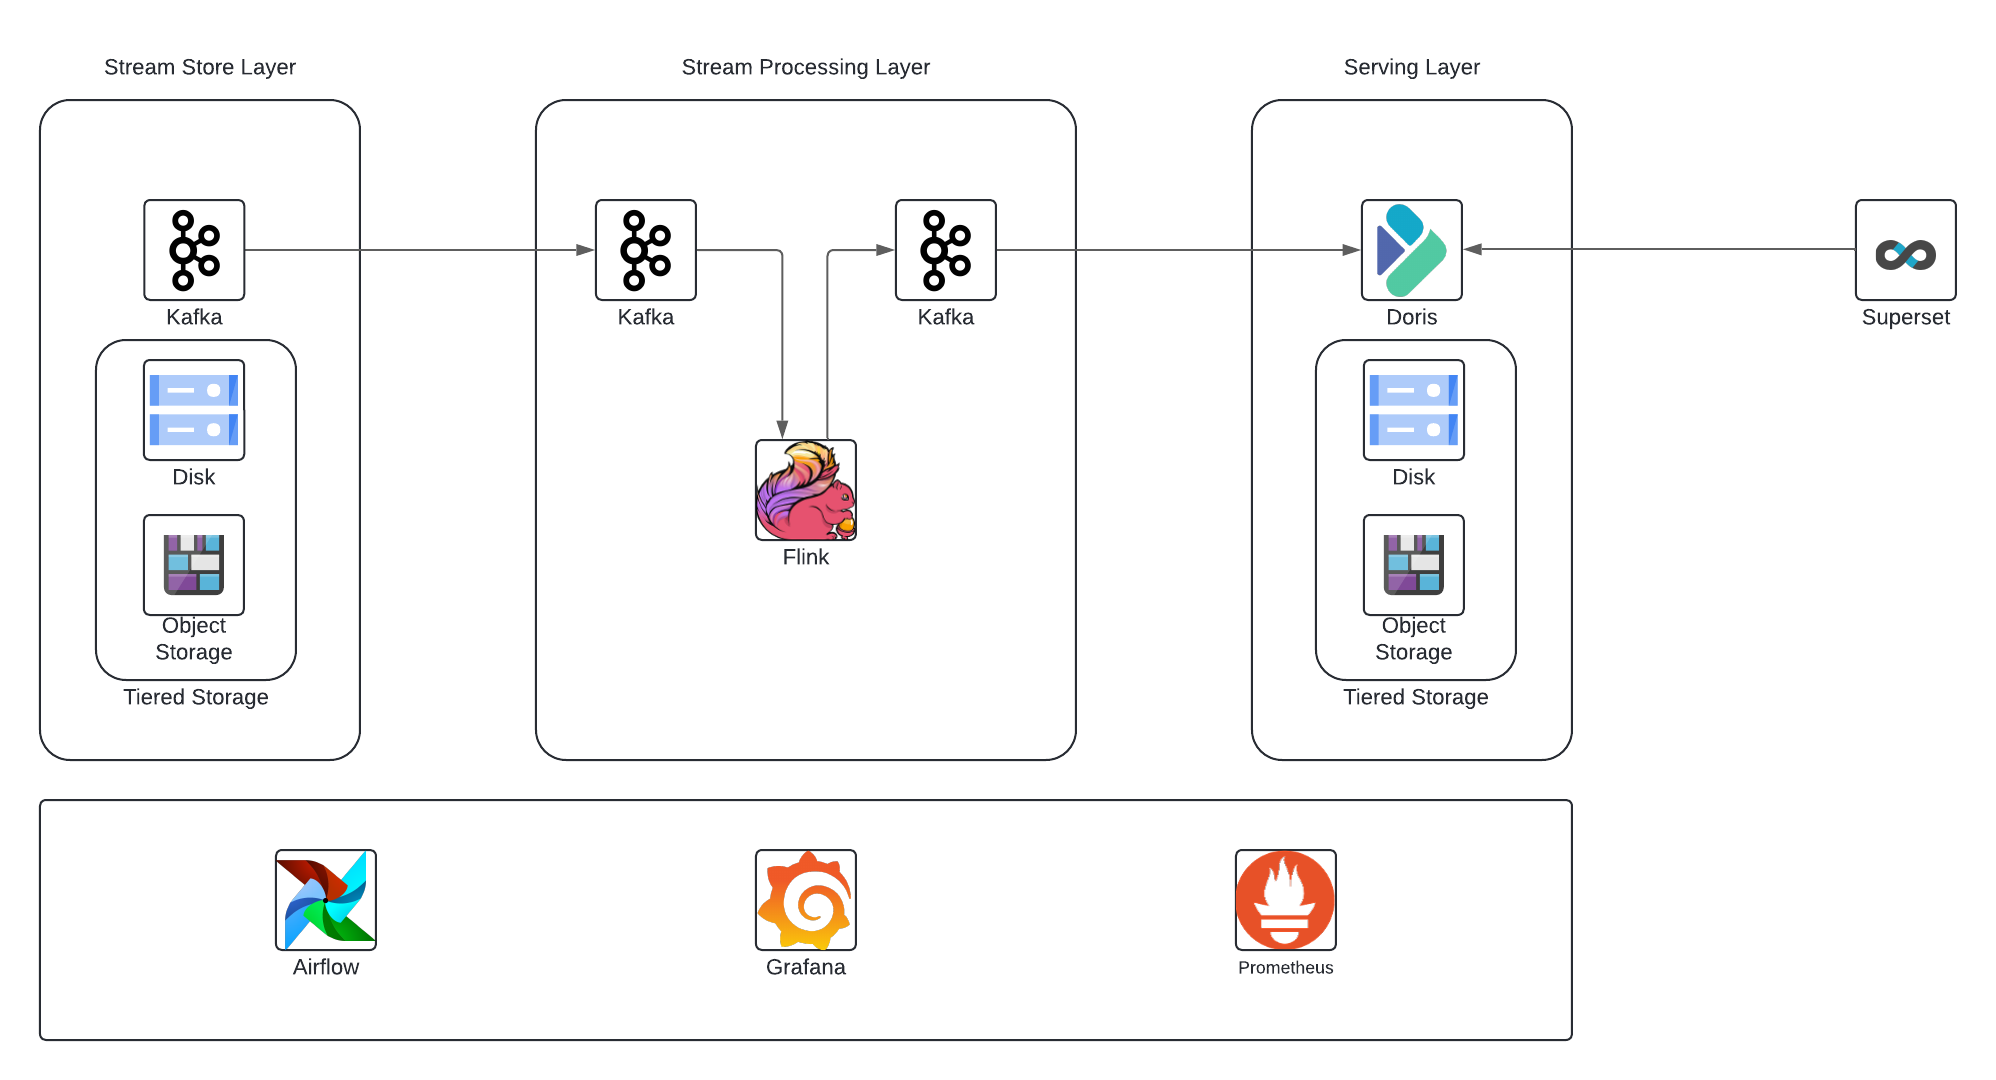
\includegraphics[width=\paperwidth]{desarrollo/Kappa.png}}
    \caption{Diagrama de la Arquitectura Kappa}
    \label{fig:des_arquitectura_kappa}
\end{figure}

\newpage

\subsection{Flujo de Procesamiento}

El siguiente es un ejemplo de uno de los trabajos de procesamiento de datos desarrollados:

\begin{lstlisting}[language=sql]
    SET 'execution.runtime-mode' = 'streaming';
    SET 'execution.checkpointing.mode' = 'EXACTLY_ONCE';
    SET 'table.local-time-zone' = 'UTC';
    SET 'execution.checkpointing.interval' = '60000';
    SET 'execution.checkpointing.timeout' = '30000';
    SET 'state.backend' = 'hashmap';
    SET 'table.exec.state.ttl' = '300000';
    SET 'parallelism.default' = '4';
\end{lstlisting}

\begin{lstlisting}[language=sql]
    -- Raw measurements table with original timestamps and device metrics
    CREATE TABLE raw_measurements (
        measurement_timestamp TIMESTAMP(3),
        measurement_type STRING,
        raw_value STRING,
        device_id STRING,
        battery DOUBLE,
        signal_strength DOUBLE,
        ingestion_timestamp TIMESTAMP(3) METADATA FROM 'timestamp' VIRTUAL,
        WATERMARK FOR measurement_timestamp AS measurement_timestamp - INTERVAL '10' SECONDS
    ) WITH (
        'topic' = 'raw.measurements',
        'connector' = 'kafka',
        'properties.bootstrap.servers' = 'kafka-1:19091,kafka-2:19092,kafka-3:19093',
        'format' = 'json',
        'json.timestamp-format.standard' = 'ISO-8601',
        'scan.startup.mode' = 'latest-offset'
    );
\end{lstlisting}
\newpage
\begin{lstlisting}[language=sql]
    CREATE TABLE enriched_measurements (
        measurement_type STRING,
        `value` DOUBLE,
        device_id STRING,
        patient_id STRING,
        
        -- Weights
        quality_weight DOUBLE,
        freshness_weight DOUBLE,
        
        -- Timestamps
        measurement_timestamp TIMESTAMP(3),
        ingestion_timestamp TIMESTAMP(3),
        enrichment_timestamp TIMESTAMP(3) METADATA FROM 'timestamp' VIRTUAL,
        WATERMARK FOR measurement_timestamp AS measurement_timestamp - INTERVAL '10' SECONDS
    ) WITH (
        'topic' = 'enriched.measurements',
        'connector' = 'kafka',
        'properties.bootstrap.servers' = 'kafka-1:19091,kafka-2:19092,kafka-3:19093',
        'format' = 'json',
        'json.timestamp-format.standard' = 'ISO-8601',
        'scan.startup.mode' = 'latest-offset'
    );
\end{lstlisting}
\newpage
\begin{lstlisting}[language=sql]
    -- Insert with quality and freshness calculations
    INSERT INTO enriched_measurements
    SELECT
        measurement_type,
        CAST(raw_value AS DOUBLE) AS `value`,
        device_id,
        REGEXP_EXTRACT(device_id, '.*_(P\d+)$', 1) AS patient_id,

        -- Quality components
        CAST((
            CASE
                WHEN device_id LIKE 'MEDICAL%' THEN 1.0
                WHEN device_id LIKE 'PREMIUM%' THEN 0.7
                ELSE 0.4
            END * 0.7 +
            CASE
                WHEN battery >= 80 THEN 1.0
                WHEN battery >= 50 THEN 0.8
                WHEN battery >= 20 THEN 0.6
                ELSE 0.4
            END * 0.2 +
            CASE
                WHEN signal_strength >= 0.8 THEN 1.0
                WHEN signal_strength >= 0.6 THEN 0.8
                WHEN signal_strength >= 0.4 THEN 0.6
                ELSE 0.4
            END * 0.1
        ) AS DECIMAL(7,2)) AS quality_weight,

        -- Combined freshness calculation
        CASE
            WHEN TIMESTAMPDIFF(HOUR, measurement_timestamp, ingestion_timestamp) <= 1 THEN 1.0
            WHEN TIMESTAMPDIFF(HOUR, measurement_timestamp, ingestion_timestamp) <= 6 THEN 0.9
            WHEN TIMESTAMPDIFF(HOUR, measurement_timestamp, ingestion_timestamp) <= 12 THEN 0.7
            WHEN TIMESTAMPDIFF(HOUR, measurement_timestamp, ingestion_timestamp) <= 24 THEN 0.5
            WHEN TIMESTAMPDIFF(HOUR, measurement_timestamp, ingestion_timestamp) <= 48 THEN 0.3
            ELSE 0.2
        END AS freshness_weight,
        
        -- Timestamps
        measurement_timestamp,
        ingestion_timestamp
    FROM raw_measurements;
\end{lstlisting}

Como se puede ver, FLink SQL permite tratar a los tópicos de Kafka como tablas, pudiendose así leer y escribir sobre ellos. 
Esto permite realizar un procesamiento de datos en tiempo real,
enriquecerlos y enviarlos a otro tópico de Kafka para su posterior procesamiento.

Para esta arquitectura se utilizaron dos conectores diferentes de Kafka. El primero, visto en los ejemplos, permite leer y escribir pero no modificar. 
Por otro lado, para las agregaciones, se utilizó \textbf{upsert-kafka} que agrega la semántica de actualización y borrado de mensajes,
que es muy útil para cuando se necesita un procesamiento incremental de la información, como es el caso de las agregaciones. 
Aunque cabe destacar que la potencia de Flink permite que se pueda hacer esto incluso para otros destinos de datos como se verá más adelante para Paimon.
Todo esto sin cambiar el código del trabajo de procesamiento. 

\newpage

\begin{lstlisting}[language=sql]
    CREATE TABLE scores (
        patient_id STRING,
        window_start TIMESTAMP(3),
        window_end TIMESTAMP(3),

        respiratory_rate_value DOUBLE,
        oxygen_saturation_value DOUBLE,
        blood_pressure_value DOUBLE,
        heart_rate_value DOUBLE,
        temperature_value DOUBLE,
        consciousness_value DOUBLE,

        respiratory_rate_score DOUBLE,
        oxygen_saturation_score DOUBLE,
        blood_pressure_score DOUBLE,
        heart_rate_score DOUBLE,
        temperature_score DOUBLE,
        consciousness_score DOUBLE,

        respiratory_rate_trust_score DOUBLE,
        oxygen_saturation_trust_score DOUBLE,
        blood_pressure_trust_score DOUBLE,
        heart_rate_trust_score DOUBLE,
        temperature_trust_score DOUBLE,
        consciousness_trust_score DOUBLE,

        measurement_timestamp TIMESTAMP(3),
        ingestion_timestamp TIMESTAMP(3),
        enrichment_timestamp TIMESTAMP(3),
        routing_timestamp TIMESTAMP(3),
        scoring_timestamp TIMESTAMP(3),
        union_timestamp TIMESTAMP(3),
        WATERMARK FOR union_timestamp AS union_timestamp - INTERVAL '10' SECONDS,
        PRIMARY KEY (patient_id, window_start) NOT ENFORCED
    ) WITH (
        'connector' = 'upsert-kafka',
        'topic' = 'scores',
        'properties.bootstrap.servers' = 'kafka-1:19091,kafka-2:19092,kafka-3:19093',
        'key.format' = 'json',
        'value.format' = 'json'
    );
\end{lstlisting}

\newpage

\begin{lstlisting}[language=sql]
    INSERT INTO scores
    SELECT * FROM (
        WITH unions as (
            ...
        )
        SELECT 
            patient_id,
            window_start,
            MAX(window_end) as window_end,

            MAX(CASE WHEN measurement_type = 'RESPIRATORY_RATE' THEN `value` END) as respiratory_rate_value,
            MAX(CASE WHEN measurement_type = 'OXYGEN_SATURATION' THEN `value` END) as oxygen_saturation_value,
            MAX(CASE WHEN measurement_type = 'BLOOD_PRESSURE_SYSTOLIC' THEN `value` END) as blood_pressure_value,
            MAX(CASE WHEN measurement_type = 'HEART_RATE' THEN `value` END) as heart_rate_value,
            MAX(CASE WHEN measurement_type = 'TEMPERATURE' THEN `value` END) as temperature_value,
            MAX(CASE WHEN measurement_type = 'CONSCIOUSNESS' THEN `value` END) as consciousness_value,

            ...

            MIN(measurement_timestamp) AS measurement_timestamp,
            MIN(ingestion_timestamp) AS ingestion_timestamp,
            MIN(enrichment_timestamp) AS enrichment_timestamp,
            MIN(routing_timestamp) AS routing_timestamp,
            MIN(scoring_timestamp) AS scoring_timestamp,
            CURRENT_TIMESTAMP as union_timestamp
        FROM TABLE(
            TUMBLE(
                TABLE unions, 
                DESCRIPTOR(measurement_timestamp), 
                INTERVAL '1' MINUTES
            )
        ) AS unions 
        GROUP BY patient_id, window_start
    ) as t;
\end{lstlisting}

\newpage
Por último, se guarda el resultado del procesamiento en \textbf{Apache Doris} directamente desde Flink.
Para esto, es necesario que la tabla en Doris haya sido creada previamente y además definir un nombre con el que llamarla en el trabajo de procesamiento.
Luego, se puede insertar los datos y Flink y Doris acordarán la forma de hacerlo. Según las pruebas realizadas, esto se hace en batches. 
El tiempo, entre que se terminó de procesar y fue insertado en Doris no fue posible de medir ya que no se encontraró una forma de definir la fecha de inserción real.

\newpage

\begin{lstlisting}[language=SQL]
    CREATE TABLE doris_gdnews2_scores (
        patient_id STRING,
        window_start TIMESTAMP(3),
        window_end TIMESTAMP(3),

        -- AVG Raw measurements
        ...

        -- Raw NEWS2 scores
        ...
        news2_score DOUBLE,

        -- Trust gdNEWS2 scores
        ...

        news2_trust_score DOUBLE,

        -- Timestamps
        measurement_timestamp TIMESTAMP(3),
        ingestion_timestamp TIMESTAMP(3),
        enrichment_timestamp TIMESTAMP(3),
        routing_timestamp TIMESTAMP(3),
        scoring_timestamp TIMESTAMP(3),

        flink_timestamp TIMESTAMP(3),
        aggregation_timestamp TIMESTAMP(3),
        PRIMARY KEY (patient_id, window_start) NOT ENFORCED
    ) WITH (
        'connector' = 'doris',
        'fenodes' = '172.20.4.2:8030',
        'table.identifier' = 'kappa.gdnews2_scores',
        'username' = 'kappa',
        'password' = 'kappa',
        'sink.label-prefix' = 'doris_sink_gdnews2',
        'sink.properties.format' = 'json',
        'sink.properties.timezone' = 'UTC'
    );
\end{lstlisting}

\begin{lstlisting}[language=SQL]
    INSERT INTO doris_gdnews2_scores
    SELECT *
    FROM gdnews2_scores;
\end{lstlisting}
\newpage
\section{Arquitectura Delta}

\subsection{Principios de Diseño}

Todo el almacenamiento de datos a largo plazo se realiza en un formato de tabla abierta, 
que combina archivos en formato Parquet con un registro de transacciones. 
Esto garantiza propiedades ACID y permite operaciones confiables en entornos distribuidos. \newline

Al utilizar object storage, se logra una separación clara entre los recursos de procesamiento y los de almacenamiento, 
lo que permite escalarlos de manera independiente. \newline

Además, múltiples clientes pueden acceder a los mismos datos de forma simultánea sin interferencias, 
incluso utilizando herramientas diferentes, siempre que sean compatibles con el formato subyacente.\newline

El formato Parquet, al ser columnar, permite ejecutar consultas SQL de manera eficiente 
y es compatible con la mayoría de los motores de análisis modernos. \newline

El procesamiento de datos se gestiona como un flujo continuo de eventos, 
donde el motor de procesamiento utiliza el log de transacciones como fuente de verdad para mantener el estado de los datos. 
Esto permite unificar el procesamiento batch y streaming en una misma arquitectura.
Como efecto secundario de esto, todos los datos son guardados para cada etapa del flujo de procesamiento. 
Esto significa que están disponibles para su fácil consumo en caso de que se quieran analizar; 
pero como contraparte, consumen más espacio de almacenamiento ya que se almacena potencialmente varias veces el mismo dato (aunque enriquecido). \newline

Además, el sistema se encarga automáticamente de optimizaciones como la compactación de archivos pequeños
y la gestión eficiente de metadatos, asegurando un rendimiento óptimo sin intervención manual.\newline

Por último, al estar basado en estándares abiertos, el sistema evita el vendor lock-in 
y permite integración con diversas herramientas de BI, machine learning y ETL.

\newpage
\subsection{Stack Tecnológico}
Para la capa de ingesta y transporte de datos se implementó \textbf{Apache Kafka}, 
un sistema de mensajería distribuido que proporciona alta durabilidad, replicación y garantía en el orden de los eventos. 
Kafka actúa como el punto de entrada de la arquitectura, permitiendo desacoplar la ingesta de datos del procesamiento 
y asegurando una capa de buffer que absorbe picos de tráfico mientras mantiene los datos disponibles para su consumo.
En este caso, Kafka se despliega en un cluster de tres nodos, con un factor de replicación de tres y un factor de partición de tres.
Por otro lado, se definió un tiempo de retención de mensajes acotado, en este caso de 7 días, para evitar la acumulación de datos
pero a su vez, asegurar la disponibilidad de los mismos para su procesamiento.\newline

El procesamiento de datos se realiza mediante \textbf{Apache Flink}, se despliega en un cluster con un nodo Job Manager 
y cinco nodos Task Manager; de forma de distribuir la carga de trabajo lo mejor posible.
En este caso, se define como punto de entrada un tópico de Kafka, para luego continuar procesando los datos, 
no utilizando Kafka sino aprovechando las capacidades de \textbf{Apache Paimon}. 
Este adopta un enfoque log-structured para las escrituras, 
lo que lo hace eficiente para cargas de trabajo de streaming con alta frecuencia de actualizaciones.\newline

Este permite tratar una tabla de datos como un flujo continuo de eventos, funcionando de forma efectiva como 
una cola de mensajes, pero con la ventaja de tener los datos materializados en un almacenamiento persistente y barato.\newline

Por último, este formato de almacenamiento permite ser leido por \textbf{Apache Doris}, un motor de análisis de datos
distribuido que permite realizar consultas SQL en tiempo real sobre grandes volúmenes de datos con una interfaz basada en MySQL.\newline

Para esto, tanto como para el uso de Flink, se necesita definir un catálogo de tablas.
Normalmente, esto podría hacerse utilizando Apache Hive, pero se optó por simplificar el sistema tanto como sea posible, 
y dado que no se necesitaba interactuar con un sistema existente; por lo que el catálogo se almacenó en Object Storage.\newline
\newpage
Esto último se logró mediante el uso de \textbf{MinIO}, un servidor de almacenamiento de objetos de código abierto que
permite almacenar datos de forma segura y eficiente, y que además es compatible con el protocolo S3 de Amazon Web Services.\newline

Esta combinación tecnológica permite implementar efectivamente los principios de la Arquitectura Delta, 
donde los datos fluyen desde las fuentes a través de Kafka, son procesados por Flink, 
almacenados en diferentes capas mediante Paimon sobre MinIO, y finalmente consultados a través de Doris, 
manteniendo en todo momento las propiedades ACID 
y permitiendo el procesamiento continuo así como análisis retrospectivos sobre datos históricos.

\newpage
\subsection{Vista de Componentes}


\begin{figure}[h]
    \makebox[\textwidth]{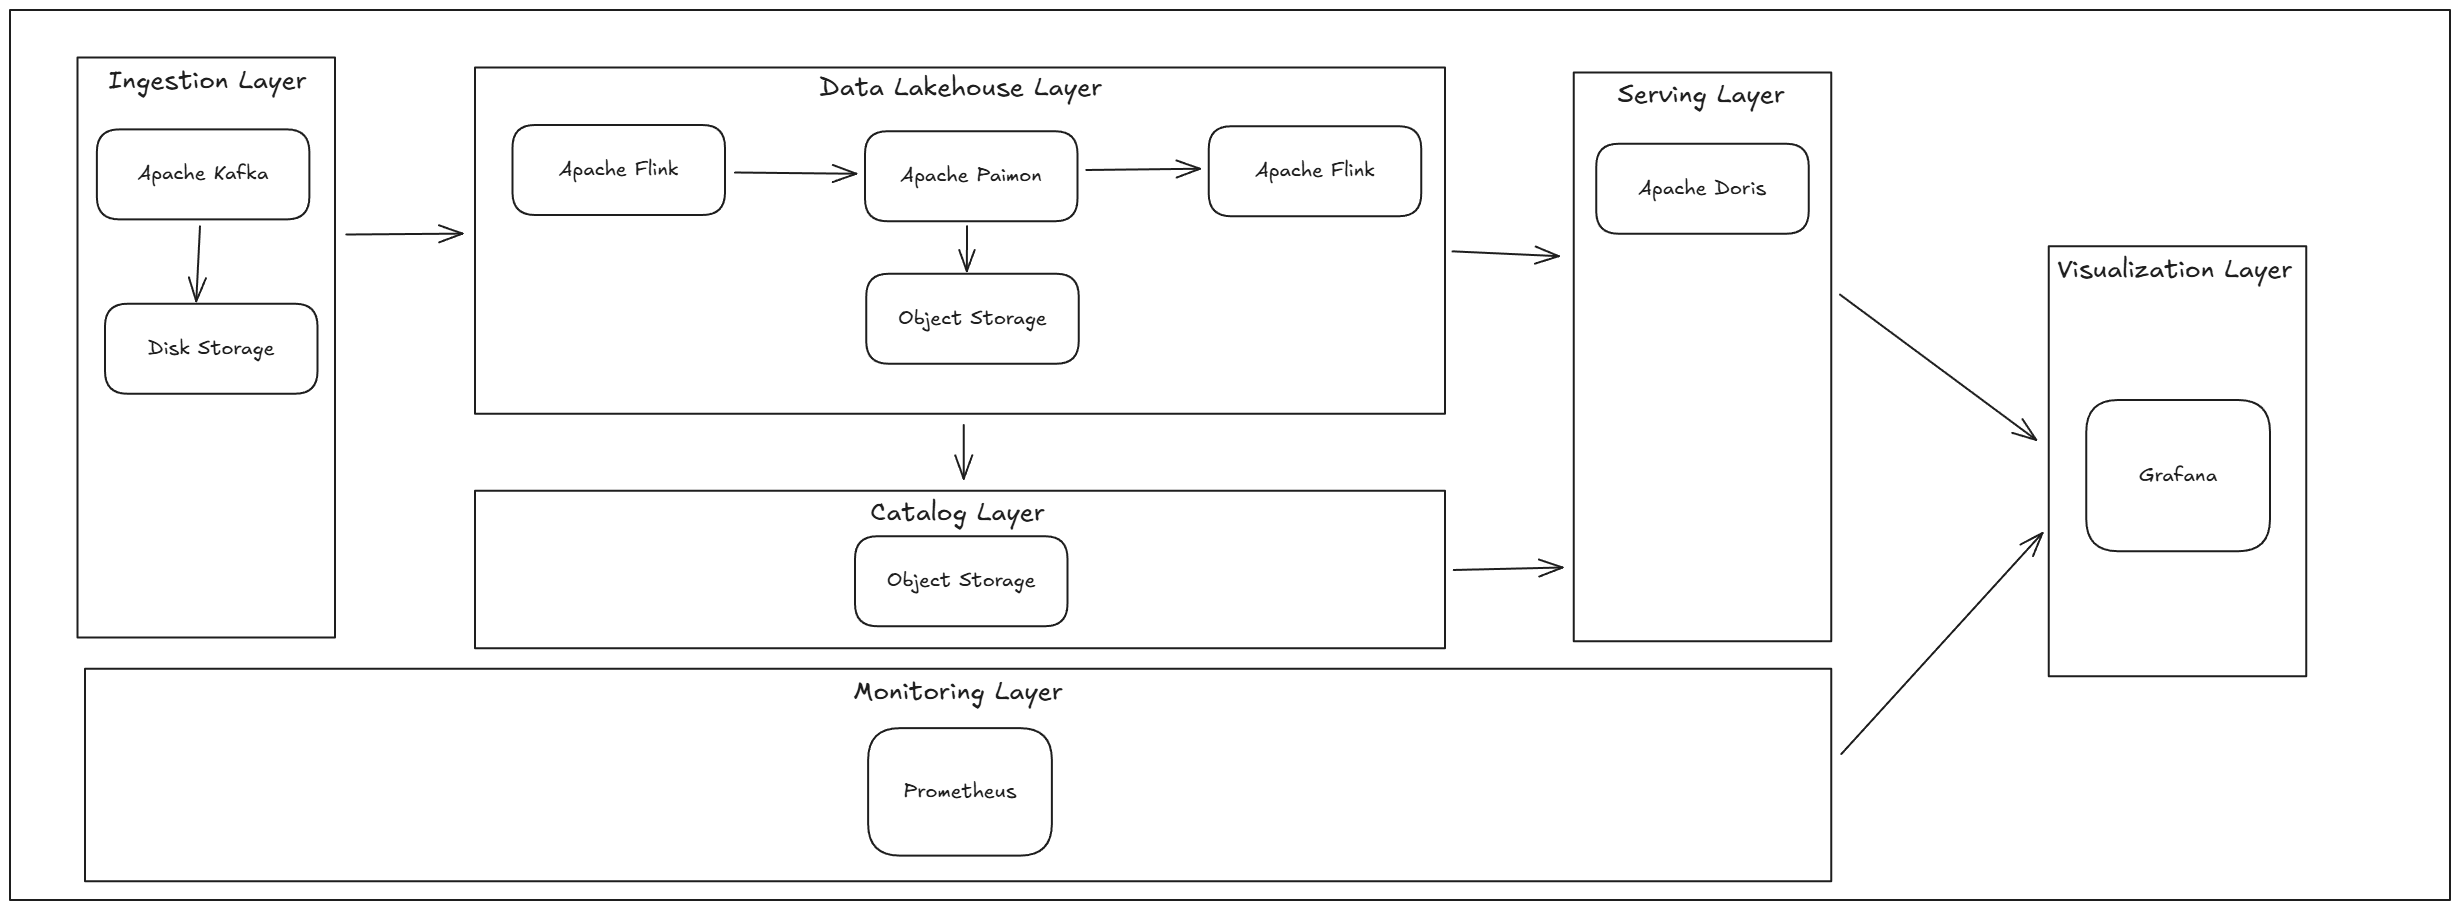
\includegraphics[width=\paperwidth]{desarrollo/Delta.png}}
    \caption{Diagrama de la Arquitectura Delta}
    \label{fig:des_arquitectura_delta}
\end{figure}

\clearpage
\newpage

\subsection{Flujo de Procesamiento}

El siguiente es un ejemplo de uno de los trabajos de procesamiento de datos desarrollados:

\begin{lstlisting}[language=sql]
    SET 'execution.runtime-mode' = 'streaming';
    SET 'execution.checkpointing.mode' = 'EXACTLY_ONCE';
    SET 'table.local-time-zone' = 'UTC';
    SET 'execution.checkpointing.interval' = '60000';
    SET 'execution.checkpointing.timeout' = '30000';
    SET 'state.backend' = 'hashmap';
    SET 'table.exec.state.ttl' = '300000';
    SET 'parallelism.default' = '2';

    CREATE CATALOG paimon WITH (
        'type' = 'paimon',
        'warehouse' = 's3://datalake/paimon',
        's3.endpoint' = 'http://minio:9000',
        's3.access-key' = 'minioadmin',  
        's3.secret-key' = 'minioadmin',
        's3.path.style.access' = 'true',
        'location-in-properties' = 'true'
    );
\end{lstlisting}

\begin{lstlisting}[language=sql]
    CREATE TABLE paimon.delta.raw_measurements (
        measurement_timestamp TIMESTAMP(3),
        measurement_type STRING,
        raw_value STRING,
        device_id STRING,
        battery DOUBLE,
        signal_strength DOUBLE,
        ingestion_timestamp TIMESTAMP(3),
        WATERMARK FOR measurement_timestamp AS measurement_timestamp - INTERVAL '10' SECONDS
    );
\end{lstlisting}

\newpage

\begin{lstlisting}[language=sql]
    CREATE TABLE default_catalog.default_database.raw_measurements (
        measurement_timestamp TIMESTAMP(3),
        measurement_type STRING,
        raw_value STRING,
        device_id STRING,
        battery DOUBLE,
        signal_strength DOUBLE,
        ingestion_timestamp TIMESTAMP(3) METADATA FROM 'timestamp' VIRTUAL,
        WATERMARK FOR measurement_timestamp AS measurement_timestamp - INTERVAL '10' SECONDS
    ) WITH (
        'topic' = 'raw.measurements',
        'connector' = 'kafka',
        'properties.bootstrap.servers' = 'kafka-1:19091,kafka-2:19092,kafka-3:19093',
        'format' = 'json',
        'json.timestamp-format.standard' = 'ISO-8601',
        'scan.startup.mode' = 'latest-offset'
    );
\end{lstlisting}

\begin{lstlisting}[language=sql]
    INSERT INTO paimon.delta.raw_measurements
    SELECT * FROM default_catalog.default_database.raw_measurements;
\end{lstlisting}

Este código muestra algunas de las características principales del uso de Flink SQL en conjunto con Paimon.
Las primeras tres reglas son las estándares para un procesamiento de streaming 
con manejo de mensajes en tiempo real y que además utilice una hora estándar para tener sincronizadas
las marcas de tiempo de todos los sistemas que intervienen.\newline

Luego se define el 'execution.checkpointing.interval' que es de los parámetros más importantes para el procesamiento de streaming,
ya que define cada cuanto tiempo se guardan los estados intermedios de los datos procesados.
Para el caso de Paimon particularmente, marca cada cuanto se impactan los datos procesados en el almacenamiento,
por lo que define que tan pronto estarán disponibles estos para su consumo.\newline

Esto afecta directamente a la latencia, por lo que es algo que se tiene que balancear fuertemente con 
los recursos del sistema para evitar retrasos en el procesamiento.\newline

\newpage

Algo importante a destacar es que si bien en este caso se define el catálogo en cada uno de los scripts, 
esto no debería ser necesario pues Flink permite definir mediante configuración sus catálogos disponibles.
Sin embargo, no fue posible configurarlo de esta manera, por lo que se optó por definirlo en cada uno de los scripts.\newline

Un último detalle a destacar, es que se define el paralelismo en 2 de modo tal que se pueda aprovechar al máximo 
las particiones del tópico de Kafka. Lo ideal sería definirlo en 3, 
pero esto no es posible por una limitante de hardware en cuanto a memoria en el nodo que ejecuta el trabajo de procesamiento.\newline

Esta primer inserción de datos que se encarga de recibir los datos en formato JSON desde el tópico de Kafka
y almacenarlos en el formato de Paimon es una de las dos grandes diferencias de esta arquitectura respecto a la anterior.
La segunda diferencia es que en este caso no es necesaria la inserción en Doris, ya que esta es sólo una herramienta que se usa para acceder a los datos pero no los almacena. 
Esto hace que el flujo de procesamiento sea más simple y liviano al no haber un tercer componente que tenga que procesar información. 
\newpage
\section{Decisiones Técnicas de Arquitectura}

En esta sección se detallan las principales decisiones de diseño arquitectónico tomadas durante la implementación del sistema,
 con foco en los aspectos de alta disponibilidad, interoperabilidad, simplicidad operativa y escalabilidad futura.

\subsection{Cluster de Kafka y ZooKeeper}
Se configuró un clúster de Kafka con 3 brokers y 3 nodos de ZooKeeper. Esta arquitectura permite:
\begin{itemize}
    \item Alta disponibilidad y tolerancia a fallos de nodos individuales
    \item Replicación de particiones con \texttt{replication.factor = 3}
    \item Tolerancia a la pérdida de hasta un nodo en cada capa (brokers o ZooKeeper)
\end{itemize}
Esta configuración es apropiada para entornos productivos y garantiza durabilidad y disponibilidad en la capa de mensajería.

\subsection{Despliegue de Apache Doris}
Se implementaron 3 nodos Backend (BE), permitiendo la distribución de datos y procesamiento paralelo. 
Sin embargo, sólo se desplegó una instancia de Frontend (FE), lo que representa un punto único de falla (\textit{Single Point of Failure}). 
En un entorno de producción, se recomienda utilizar múltiples nodos FE en configuración maestro-seguidor para garantizar disponibilidad continua del servicio de consultas y acceso al catálogo.

\subsection{Catálogo de Datos}
Se optó por utilizar un catálogo basado en sistema de archivos (object storage) para el manejo de tablas analíticas, sin integración con Hive Metastore. 
Esta decisión simplificó la infraestructura y redujo la complejidad operativa. Si bien esta elección limita la interoperabilidad entre motores de procesamiento, 
resulta adecuada para soluciones encapsuladas donde no se requiere acceso simultáneo desde múltiples tecnologías.

\subsection{Coordinación de Procesamiento}
Se utilizó una única instancia de JobManager de Apache Flink. Esta configuración es suficiente para entornos controlados, pero representa una limitación en cuanto a tolerancia a fallos. 
En escenarios reales, se recomienda implementar Flink en modo de alta disponibilidad, utilizando múltiples JobManagers (activo y pasivos), 
un backend compartido para almacenamiento de estado (por ejemplo, S3), 
y un coordinador de liderazgo como ZooKeeper.

\subsection{Justificación General}
Las decisiones tomadas responden a un enfoque de prototipo funcional, priorizando la validación de las arquitecturas Kappa y Delta en condiciones controladas. 
Se buscó un equilibrio entre fidelidad técnica y simplicidad de despliegue, permitiendo reproducibilidad y flexibilidad sin incurrir en la complejidad de un entorno productivo completo.

\newpage
\chapter{Resultados}

\section{Análisis Comparativo}

\subsection{Aspectos Técnicos}

\subsection{Aspectos Operativos}

\subsection{Aspectos de Costo}

\subsection{Casos de Uso Óptimo}

\subsection{Limitaciones}

\section{Evolución a Futuro}

\subsection{Tecnologías Emergentes}

\subsection{Mejoras de Diseño}
\chapter{Conclusiones}
Contenido del capítulo...



% # 7. Future Research Directions

% ## 7.1 Parameter Optimization

% ### Time Windows and Degradation Rates
% - Empirical validation of freshness weight decay rates
% - Patient-specific adaptation of maximum time windows
% - Impact of circadian rhythms on measurement validity periods
% - Optimization of quality weight component ratios

% ### Alert Thresholds
% - Machine learning approaches for dynamic threshold adjustment
% - Population-based threshold optimization
% - Context-aware alert modification
% - Alert fatigue reduction strategies

% ## 7.2 Quality Assessment Enhancement

% ### Device Quality Metrics
% - Validation protocols for new device types
% - Cross-device correlation studies
% - Environmental impact on device accuracy
% - Long-term drift detection methods

% ### Measurement Conditions
% - Automated detection of measurement interference
% - Impact of patient activity on measurement quality
% - Environmental factor quantification
% - Multi-sensor fusion for condition assessment

% ## 7.3 Clinical Validation

% ### gdNEWS2 Effectiveness
% - Comparison with traditional NEWS2 in clinical settings
% - Impact on patient outcomes
% - False positive/negative rate analysis
% - Cost-benefit analysis of implementation

% ### Score Adjustment Mechanisms
% - Alternative degradation models
% - Non-linear quality weight impacts
% - Parameter interdependency effects
% - Confidence level optimization

% ## 7.4 System Optimization

% ### Performance Parameters
% - Optimal measurement frequencies
% - Data validation thresholds
% - Alert buffer periods
% - System recovery procedures

% ### Integration Capabilities
% - Multi-device synchronization methods
% - Data format standardization
% - Legacy system compatibility
% - Real-time processing optimization

% These research directions aim to enhance the system's clinical validity while maintaining its practical implementability. Each area represents an opportunity for focused studies that could lead to meaningful improvements in remote patient monitoring capabilities.

% Anexos
\appendix

\chapter{Repositorio de código}

Se definireron tres repositorios de código para el desarrollo de la arquitectura Kappa y Delta.
El primero de ellos es el repositorio de la arquitectura Kappa, que contiene el código de procesamiento de datos y la configuración de los componentes.
El segundo es el repositorio de la arquitectura Delta, que contiene el código de procesamiento de datos y la configuración de los componentes.
El tercero es el repositorio del generador de datos sintéticos que se utilizó para realizar las pruebas de carga y estrés.

El código de cada uno de los repositorios se encuentra disponible en el siguiente enlace:

\begin{itemize}
    \item \url{https://github.com/Rekeyea/Tesis-Kappa}\\
    \item \url{https://github.com/Rekeyea/Tesis-Delta}\\
    \item \url{https://github.com/Rekeyea/Tesis-SynthDS}\\
\end{itemize}


% Bibliografía
\printbibliography
\end{document}